\documentclass[10pt]{article} % For LaTeX2e
\usepackage{tmlr}
% For camera-ready (after acceptance), switch to: \usepackage[accepted]{tmlr}
% For preprint/arXiv posting (de-anonymized), switch to: \usepackage[preprint]{tmlr}

\input{math_commands.tex}

\usepackage{hyperref}
\usepackage{url}
\usepackage{amsmath}
\usepackage{amssymb}
\usepackage{booktabs}
\usepackage{graphicx}

\title{Selection-Induced Optimism in Hidden-State Hallucination Detection: A
Code-Verified Taxonomy, and Why Severity Tracks Candidate Count and
Operating Point Rather Than Mechanism}

% Authors must not appear in the submitted version -- tmlr.sty hides this
% automatically as long as neither [accepted] nor [preprint] is active.
% This public/anonymized copy additionally carries a placeholder author block,
% matching the anonymous-submission convention used in kernel-metadata.json.
\author{\name Anonymous Author \email anonymous@example.com \\
      \addr Anonymous Institution}

\begin{document}

\maketitle

\begin{abstract}

We study \emph{selection-induced optimism} in hidden-state
hallucination-detection pipelines: numeric inflation of a reported metric
caused by choosing a checkpoint, layer, threshold, or hyperparameter using
the same data --- or a statistic derived from it --- later used to report
performance. We identify five structurally distinct selection surfaces
across two published pipelines and our own, three of them verified
directly against pinned third-party source code: full-dataset
fit-then-score feature leakage; cross-validation-based layer selection
reported as held-out performance; training-loop checkpoint and scheduler
coupling to a reused validation fold; test-set-driven best-layer
selection; and test-set-tuned decision thresholds.

\textbf{Contrary to an earlier framing of this line of work, severity
does not differ sharply by which mechanism is responsible.} Measured with
matched controls --- a placebo baseline, budget- and seed-matched clean
conditions, and a bias-corrected, label-free calibration guardrail ---
every mechanism with a code-verified AUROC-scale estimate lands in a
narrow band: $+0.027$ (SD $0.021$, $p=0.009$) for CV-based layer
selection, $+0.0009$ to $+0.0034$ for per-fold checkpoint selection on
the primary synthetic sweep, $+0.0054$ (BCa 95\% CI
$[+0.0032,+0.0100]$, 24 published result files) for test-set-driven
best-layer selection, and exactly zero for test-set threshold selection,
which is threshold-free-metric-invariant by construction while inflating
F1 and accuracy by $+0.021$ to $+0.034$ ($p<10^{-31}$).

Severity instead tracks two continuous, mechanism-independent
quantities. Holding the mechanism fixed, inflation grows with the number
of candidates selected among (well fit by $a+b\ln K$, $R^2=0.970$;
notably \emph{not} by the extreme-value form
$c\,\sigma_{\text{val}}\sqrt{2\ln K}$, which gives $R^2=-0.399$ when fit
as stated) and falls sharply with the model's operating point --- by a
factor of $48.6\times$, from $+0.0093$ at AUROC$_0=0.70$ to $+0.0002$ at
$0.985$. That single relationship moves severity more than any
difference we measure between mechanisms, and explains why several
estimates here come out near zero: they were measured on tasks already
running near the ceiling.

While deriving these estimates we twice found our own measurement
instrument committing the very pattern this paper audits for --- first a
full-dataset calibration transform evaluated across the split it was fit
on, then a residual label-conditional step inside the fix for it --- and
replaced both with a fully label-free calibration that reaches chance
exactly at zero separation.

We release a code-verified taxonomy, this severity relationship, the
label-free calibration guardrail, and an extension of the Kapoor \&
Narayanan / REFORMS leakage checklists. We also test whether the
checklist can be automated: a regex scanner over 7 repositories yields
zero true positives and misses both known bugs, for two causes we
diagnose specifically rather than generalize from. \textbf{We do not
claim} any field-wide prevalence estimate, any deployment-impact
estimate, or that our largest single figure ($+0.19$ AUROC, Case Study 1)
is verified --- no artifact supporting it ships with this paper, and we
exclude it from every comparison above.

\end{abstract}

\section{Introduction}

Detecting hallucination by probing an LLM's internal hidden states is one
of the most active subfields in LLM reliability research: a linear probe
is cheap to train and needs no additional model calls, and reported
AUROCs are often striking -- 0.90 or higher, sometimes a perfect 1.000.
This is also a setting with few samples and many dimensions (hundreds of
samples, thousands of hidden dimensions), where high reported numbers
should invite scrutiny of the evaluation protocol that produced them.

This paper began by accident. While building our own hidden-state
hallucination detector (HaRP, targeting Qwen2.5-3B), we found and fixed a
nested-cross-validation leakage bug in our own evaluation. That raised a
question: is this an isolated mistake, or a structural hazard the broader
literature shares? We find five \emph{distinct} mechanisms by which
evaluation labels can leak into a reported metric, and verify three of
them (Mechanisms 3-5) directly against pinned commits of two externally
published, code-available pipelines.

\textbf{A correction to this line of work's own earlier framing.} An
earlier version of this paper argued that severity ``differs sharply by
mechanism, not by pipeline.'' Having now measured each mechanism against
matched controls --- a placebo baseline, budget- and seed-matched clean
conditions, and a bias-corrected calibration guardrail --- we no longer
believe that, and this version says so. Every mechanism here with a
code-verified AUROC-scale severity estimate produces inflation in a
narrow band of roughly $0.000$ to $0.027$ AUROC. What severity
\emph{does} track, strongly and mechanism-independently, is two
continuous quantities: the number of candidates selected among, and the
operating point the pipeline runs at. Holding the leakage mechanism
fixed and varying only the task's calibrated difficulty moves the
inflation by a factor of $48.6\times$ --- from $+0.0093$ at AUROC$_0=0.70$
to $+0.0002$ at $0.985$ --- which is larger than any difference we
measure \emph{between} mechanisms. That relationship, previously buried
in an appendix, is promoted here to a headline finding (§5).

\textbf{Contributions:}
\begin{enumerate}
\item A five-mechanism taxonomy of label-information leakage specific to
   hidden-state probing pipelines, with three of the five verified
   directly against pinned third-party source code, not inferred from
   methodology sections.
\item \textbf{The severity relationship:} evidence that inflation in this
   setting is governed by candidate count ($\text{gap}=a+b\ln K$,
   $R^2=0.970$) and, far more strongly, by operating point (a
   $48.6\times$ decline from AUROC$_0=0.70$ to $0.985$), rather than by
   which of the five mechanisms is responsible (§5).
\item A quantified CV-based layer-selection optimism bias in one of our
   own pipelines (GUARDIAN), including a full 32-layer decomposition and
   a randomization-based correction showing the original 18.8-point
   headline gap is almost entirely an artifact of a non-random
   train/held-out split, leaving a small but statistically significant
   selection-specific penalty ($+0.027$, SD $0.021$, $p=0.009$) once
   correctly isolated --- plus a small shipped derived artifact
   (\texttt{code/48}, \texttt{code/51}) that lets a reader recompute
   every one of those numbers without the original 171\,MB hidden-state
   cache.
\item A controlled reconstruction of Mechanism 3 (per-fold checkpoint
   selection) calibrated via a closed-form Fisher-ratio/AUROC identity,
   with an explicit alternative-confound control whose own limited power
   we quantify rather than assert, and a fidelity extension modelling the
   audited trainer's actual LR-scheduler and early-stopping coupling.
\item A directly-measured, CI-bounded winner's-curse estimate for
   Mechanism 4 from 24 published per-layer/per-seed result files, with
   its ceiling-saturated and non-saturated subsets reported separately.
\item A quantification of Mechanism 5 showing it leaves AUROC exactly
   unaffected by construction while materially inflating every
   threshold-dependent metric the same pipeline reports alongside it.
\item A non-tautological calibration guardrail for synthetic severity
   harnesses (\texttt{code/sanity\_checks.py}), built after two of this
   paper's own generators were found to have silently mislabelled their
   operating points.
\item A checklist synthesizing all five mechanisms into actionable
   questions, extending the Kapoor \& Narayanan and REFORMS leakage
   checklists, plus a negative automation result whose specific failure
   causes we diagnose rather than generalize from.
\end{enumerate}

\textbf{What we do not claim.} We give no prevalence estimate for any of
these mechanisms across the literature: the repositories examined here
were found by targeted search for exactly this failure class, not
sampled. We give no deployment-impact estimate, having no
deployment-volume or review-cost data for any audited system. And we are
explicit about one case study (Case Study 1) whose number we could not
re-verify from the artifact submitted with this paper (§4).

\section{Related Work}

\textbf{General methodological leakage.} Leakage -- evaluation-target
information influencing a reported metric -- is well documented in data
mining (Kaufman et al. 2012) and in model-selection statistics:
cross-validation-based hyperparameter or feature selection is optimistic
unless nested inside the outer evaluation loop (Varma \& Simon 2006). Case
Studies 2 and 4 are direct instances of this general phenomenon in
hidden-state probing; Case Studies 1 and 3 are more specific to the
two-stage feature-extraction-then-classification structure common in this
literature. To our knowledge, no prior work names this as a distinct
pattern here.

\textbf{Kapoor \& Narayanan's cross-field leakage taxonomy.} The closest prior
art to this paper's central move is Kapoor \& Narayanan (2023), who
survey leakage across 17 scientific fields and 294 papers and propose an
8-type taxonomy: L1.1 (no test set), L1.2 (pre-processing computed on
train+test combined), L1.3 (feature selection on train+test), L1.4
(duplicates across the split), L2 (illegitimate/proxy features), L3.1
(temporal leakage), L3.2 (non-independence between train and test
samples), and L3.3 (test distribution not matching the distribution of
scientific interest). Mapping this paper's five mechanisms onto that
taxonomy: Mechanism 4 (test-set-driven best-layer selection) and
Mechanism 5 (test-set-driven threshold selection, §5) are both direct
instances of \textbf{L1.3} (feature/model selection performed on
train${+}$test rather than on training data alone) -- the test set is
reused for a modeling decision (which layer, which threshold) and then
for the reported metric, leaving no genuinely held-out data behind that
decision. (An earlier draft of this paper mapped both to L1.1, ``no test
set'' -- that was wrong: these pipelines do construct a test split and do
train on a disjoint set; what they do illegitimately is \emph{select}
using the test split, which is precisely L1.3's scope, not L1.1's.)
Mechanism 1 (full-dataset
fit-then-score feature leakage) is an instance of L1.2, generalized from
a preprocessing statistic to an entire fitted feature-extraction model.
Mechanism 3 (per-fold checkpoint-selection leakage) is a narrower-bandwidth
variant of the same L1.2 pattern, restricted to which training iterate is
kept rather than which preprocessing statistic is used. Mechanism 2
(CV-based layer/hyperparameter selection optimism, i.e.\ Varma \& Simon's
problem) does not map cleanly onto any single one of Kapoor \& Narayanan's
eight leaf types -- it is closest in spirit to L1.2/L1.3 but is really a
distinct, model-selection-specific pattern their taxonomy does not name
explicitly, even though they cite the general model-selection-optimism
literature elsewhere. This is itself informative: three of this paper's
five mechanisms are genuine instances of an existing, general taxonomy
built for a wider scientific audience, while the CV-based
architecture/hyperparameter-selection pattern this paper's Case Study 2
documents is not explicitly one of the eight named types anywhere in
that taxonomy -- consistent with this paper's claim that hidden-state
hallucination probing's specific two-stage structure surfaces at least
one leakage pattern general cross-field taxonomies do not yet enumerate
by name.

\textbf{Benchmarking against REFORMS and the ML Reproducibility Checklist.}
Two further external standards, both broader than a leakage-specific
taxonomy, let us check whether this paper's own checklist (\S5) covers
ground those standards separately consider load-bearing. REFORMS (Kapoor
et al. 2024, \emph{Science Advances}) is a 32-item, 8-module consensus
checklist for ML-based science: study goals (3 items), computational
reproducibility (5), data quality (7), data preprocessing (3), modeling
(6), data leakage (3), metrics and uncertainty quantification (3), and
generalizability and limitations (2). Its dedicated data-leakage module
covers exactly three questions -- train/test separation, dependencies
between train and test instances, and feature legitimacy -- all three of
which are subsumed by this paper's five-mechanism taxonomy, and Mechanism
2 (CV-based layer/hyperparameter-selection optimism) again falls outside
this module's scope for the same reason it falls outside Kapoor \&
Narayanan's eight leaf types: REFORMS' data-leakage module, like the
cross-field taxonomy, treats train/test separation and feature
legitimacy as the leakage surface, not iterative model/architecture
selection against a validation signal. REFORMS' other seven modules,
however, cover reporting practices this paper does not itself audit
(study-goal framing, uncertainty quantification beyond the specific
severity estimates reported here, external-validity discussion) --
useful context for readers applying both instruments together, since
neither is a superset of the other. The NeurIPS Machine Learning
Reproducibility Checklist (Pineau et al. 2021, \emph{JMLR}) is reporting-
practice-oriented rather than leakage-specific: its four sections (all
models/algorithms presented; any theoretical claims; all datasets used;
all experiments) ask whether code, hyperparameters, dataset statistics,
compute budgets, and multi-seed variance are disclosed, none of which
individually detects a leakage bug the way REFORMS' or this paper's own
checklists attempt to. This paper's own reproducibility practice (full
per-seed result arrays, vendored external repositories, BCa
bootstrap/permutation tests on every severity gap) satisfies the bulk of
the Pineau checklist's disclosure-oriented items as a byproduct of the
statistical rigor already required for the severity claims themselves,
but that checklist would not, on its own, have caught any of the eleven
issues this paper's own Appendix A documents finding and fixing in its
own instrument -- consistent with this paper's overall argument that
reporting-practice checklists and leakage-detection checklists are
complementary, not interchangeable, and that a paper can satisfy the
former while still committing the latter.

\textbf{Calibration and benchmark-construction critiques.} A large, separate
literature asks whether LLM confidence is calibrated to correctness
(surveys, hidden-state-based confidence estimation, conformal-prediction
guarantees); this work treats the evaluation protocol as given, whereas
our contribution sits upstream of it -- an inflated AUROC corrupts any
downstream calibration analysis built on it. Closer to our concern,
PARALLAX (arXiv 2605.17028) audits 22 detection methods across 12 models
and 6 corpora and finds four of six corpora leak the ground-truth answer
directly into the input prompt; once controlled for, most baselines fall
to near chance. This is independent, larger-scale evidence that the
field's reported AUROCs are frequently protocol or construction
artifacts, though PARALLAX's mechanism (benchmark construction) is
distinct from all five mechanisms documented here (each of which concerns
a downstream selection step, not the benchmark's own construction).
Separately, surface-form correctness metrics (ROUGE-L, exact match) are
known to diverge from LLM-judge or human factual-correctness judgments --
a related but distinct label-quality concern this paper does not address.
Fixing the leakage patterns we identify does not, by itself, address
label-quality or benchmark-construction problems in the underlying
dataset.

\textbf{Pretraining-data contamination.} A separate 2023-2026 thread asks
whether a benchmark's answers appeared in an LLM's pretraining corpus
(Shi et al. 2024; Golchin \& Surdeanu 2024; Sainz et al. 2023) -- a
different failure mode from ours: contamination concerns what the model
has already seen, not whether a downstream selection step used test-set
signal after the model was already fixed. The two are complementary and,
in principle, additive; we do not audit our four case studies' benchmarks
for contamination.

To our knowledge, no prior paper both (a) names and distinguishes
multiple, structurally different label-leakage mechanisms specific to
hidden-state probing pipelines, and (b) quantifies their relative
severity via controlled reconstruction rather than assuming all leakage
is equally damaging.

\section{Method: How These Case Studies Were Selected and Verified}

Two case studies (§4.1-4.2) come from our own prior work, where we had
full access to code, data, and commit history. The external case studies
(§4.3-4.4) required three things: a real, runnable public code
repository, verified directly via the repository host, not taken on
faith from the paper's text; a reported AUROC in the range that warrants
scrutiny (0.90 or higher); and an evaluation protocol whose leakage risk
we could assess by reading the actual training/evaluation code, not just
a methodology section. We did not limit the search to K-fold setups
specifically, since one candidate paper's bug (§4.4) lives in a single
train/val/test split with no K-fold structure at all -- ``avoid K-fold'' is
not itself a fix for this family of hazards.

\section{Four Case Studies}

\textbf{Evidentiary status --- read this before any severity number below.}
These four case studies are \emph{not} equally verifiable by a reader of
this artifact, and we grade them explicitly rather than presenting all
four numbers on the same footing.

\begin{itemize}
\item \textbf{Case Studies 3 (MultiHaluDet) and 4 (quantized-LLM paper)
  --- fully verifiable here.} External, published, code-available
  systems. Their leaks are demonstrated against pinned commits of
  publicly released third-party code vendored into this artifact, and
  every audit script and result JSON behind their severity numbers ships
  with it.
\item \textbf{Case Study 2 (GUARDIAN) --- verifiable here from a derived
  artifact.} This paper's own prior, unpublished pipeline. The raw
  hidden-state cache it was originally computed from is a 171\,MB file
  too large to ship, so \texttt{code/48} now also emits a small
  ($\sim$1\,MB) derived artifact --- per-layer, per-sample
  cross-validation fold assignments and probe scores for all 32 layers,
  for the sequential split, the reversed split, and all 8 randomized
  reps --- and \texttt{code/51} recomputes every number this paper
  reports for Case Study 2 from that artifact alone and asserts
  agreement with the committed JSON.
\item \textbf{Case Study 1 (HaRP) --- \emph{not} independently
  re-verifiable from this artifact.} Its $+0.19$ figure is reported from
  our own prior work; the training scripts and logs that produced it are
  not included here and we were unable to reconstruct them for this
  submission. We keep the case study because the \emph{mechanism} it
  illustrates is real, clearly described, and the origin of this
  paper --- but we do not use its number as evidence, do not include it
  in the abstract's severity range, and do not compare it against the
  code-verified numbers. A reader should treat it as a narrative
  account, not a measurement.
\end{itemize}

Neither HaRP nor GUARDIAN was run through the automated scanner in §5,
since both were built and their leaks discovered before that scanner
existed.

\subsection{Case Study 1 (mechanism only; number not re-verifiable from this artifact): Full-dataset fit-then-score leakage — HaRP}

[See \texttt{draft/worked\_examples.md}, Case Study 1, for full detail.]

\textbf{Evidentiary status: the numbers in this subsection are reported
from our own prior work and are not reproducible from the materials
submitted with this paper.} No script, log, or result file supporting
them is included in this artifact. They are stated for completeness,
because this bug is what started this paper, and because the mechanism is
worth naming; they are excluded from the abstract's severity range and
from every cross-mechanism comparison in this paper.

HaRP's Group-C representation feature \texttt{probe\_conf} came from a
logistic-regression probe fit on all 700 samples, which then scored those
same 700 samples; only afterward did this feature enter a separate outer
5-fold cross-validation loop for the downstream failure estimator. This is
nested-CV leakage in its cleanest form: the ``held-out'' fold's feature was
manufactured by a model that had already seen every label, including that
fold's own.

\textbf{Quantified effect.} A+B+C AUROC under 5-fold CV: 0.9620 (leaked) versus
0.7714 (fixed, out-of-fold) -- a \textbf{+0.1906} inflation. \texttt{probe\_conf}
alone: in-sample AUROC 1.0000 versus proper out-of-fold AUROC 0.7573,
independently cross-checked against a separately-obtained cross-validated
AUROC of 0.7583 (agreement within 0.001).

\textbf{Fix:} refit both the probe and the class centroids per fold, using
only that fold's training indices, scoring only the held-out indices.

\subsection{Case Study 2 (selection-specific severity $+0.027$ AUROC after correction; original 18.8-point headline retracted): CV-based layer-selection optimism — GUARDIAN}

[See \texttt{draft/worked\_examples.md}, Case Study 2, for full detail.]

GUARDIAN selects its detection layer -- L11 of 32, on Mistral-7B -- by
argmax of a 5-fold cross-validated AUROC across all layers, then reports
that same CV number as the model's performance.

\textbf{Quantified effect.} CV-selection AUROC at L11: 0.804. True held-out
AUROC at L11 (trained on the first 400 samples, tested on a separate,
never-selection-touched 300): \textbf{0.616} -- an 18.8-point gap. Which layer
counts as ``optimal'' also depends on the selection rule itself: argmax
train-split CV picks L11; argmax all-data AUROC picks L19 instead.

\textbf{Fix:} after CV-based selection, evaluate exactly once more on a
disjoint held-out set that played no role in the selection.

\textbf{Full 32-layer decomposition.} An earlier version of this section
disclosed this as unavailable (``no per-layer data exists to decompose
where the gap concentrates''). That was incorrect: GUARDIAN's own raw
hidden-state cache contains the complete (700, 32, 4096) Mistral-7B
representations -- all 700 samples (the 400-sample CV pool and the
300-sample held-out set) at full dimensionality, every layer, not just
L11. \texttt{code/48\_case\_study\_2\_layer\_decomposition.py} repeats the
identical CV-vs-held-out comparison at all 32 layers under GUARDIAN's own
sequential \texttt{H[:400]}/\texttt{H[400:]} split (sanity-checked to
reproduce the published L11 numbers exactly: CV$=0.804$,
held-out$=0.616$). Under this split, the mean optimism gap across all 32
layers is $+0.192$ (SD $0.053$), statistically indistinguishable from
L11's own $+0.188$, and $18$ of the other $31$ layers show a
\emph{larger} gap than L11.

\textbf{Correction: the sequential split confounds selection optimism with
a population-difference artifact.} A subsequent adversarial review of this
very analysis found that GUARDIAN's \texttt{H[:400]}/\texttt{H[400:]}
split is a fixed slice of whatever order the dataset happens to store
samples in, not a random partition -- and the two halves are separable by
a hidden-state probe at AUROC $0.734$--$0.776$, i.e.\ they are
systematically different populations, not exchangeable draws. The
quantity that isolates selection optimism specifically is the
\emph{selection-specific component}, gap-at-the-selected-layer minus the
mean gap across all 32 layers, evaluated at whichever layer that split's
own CV-argmax actually selects (a second review caught that an earlier
version of this correction hardcoded L11 for every check, including
randomized reps that select a different layer -- fixed to use each
split's own selection). Under GUARDIAN's own sequential split, L11 is
selected and this component is $-0.004$ -- indistinguishable from zero,
meaning the 18.8-point gap is not disproportionately concentrated at
the selected layer at all once the population-difference confound is
present in every layer equally. Reversing which half is used for
selection (\texttt{H[400:]} selects, \texttt{H[:400]} held out) selects a
different layer entirely (L17, not L11) and gives a component of
$+0.074$ -- a large swing in both which layer is picked and what the
component measures, itself direct evidence that the sequential-split
number is tracking an artifact of split order, not a stable property of
the selection procedure. Recomputing under $8$ randomized stratified
$400/300$ splits (never touching the sequential order), each rep
evaluated at its own selected layer (which varies rep to rep: L10, L11,
L12, L14, L16, L18, L19, L19), gives a mean selection-specific component
of $+0.027$ (SD $0.021$; one-sample $t=3.60$, $p=0.0087$; Wilcoxon
$p=0.023$) -- small but, for the first time, correctly measured and
statistically distinguishable from zero, about $7\times$ smaller than
the sequential split's apparent $+0.188$. Separately, the \emph{general}
CV-vs-held-out gap averaged across all 32 layers (not the
selection-specific component) is $+0.192$ under the sequential split but
only $-0.005$ (SD $0.073$) under the same randomized splits --
indistinguishable from zero. \textbf{The corrected conclusion reverses,
not just narrows, the original claim}: the ``large, real, $\sim$19-point
gap present at essentially every layer'' was itself entirely an artifact
of the sequential split's population-difference confound -- under a
proper random partition there is no general CV-vs-held-out optimism in
this setup at all. What survives is narrower but genuine: a small
($+0.027$), statistically significant, specifically
selection-attributable penalty from CV-based argmax-over-layers
selection -- about $7\times$ smaller than GUARDIAN's original headline
number, and now isolated from the population-difference artifact that
previously made it impossible to tell the two apart. Full results, all
three splits and per-rep selected layers:
\texttt{results/case\_study\_2\_layer\_decomposition.json}.

\subsection{Case Study 3 (severity small: $+0.0009$ to $+0.0034$ AUROC on the primary synthetic sweep): Per-fold checkpoint-selection leakage — MultiHaluDet}

[See \texttt{draft/case\_study\_multihaludet.md} for full code excerpts. Appendix A
documents the calibration/confound-detection process and additional
robustness checks behind this section's numbers.]

MultiHaluDet (arXiv 2605.24919; repo \texttt{github.com/alvi-uiu/MultiHaluDet},
pinned at commit \texttt{c7597518}) reports up to 98.55% AUROC detecting
hallucination from Mistral-7B/LLaMA-2-7B hidden states. Its training code
(\texttt{run\_pipeline.py::stage\_2\_3\_train\_oof},
\texttt{src/training/trainer.py::train\_deep\_model\_fold}) selects each inner
fold's kept checkpoint by argmax validation AUROC on that same fold, then
stores that fold's features as ``out-of-fold'' for a downstream
meta-learner. The checkpoint choice is a function of the validation
fold's own labels; unlike Case Study 1, only the \emph{checkpoint selection},
not gradient descent itself, sees the fold's labels.

\textbf{Quantifying it.} Re-running MultiHaluDet's actual 7B-scale pipeline was
outside this paper's compute budget, so we built a synthetic
reconstruction mirroring its training loop exactly (5-fold structure,
best-val-AUC checkpoint logic, OOF-feature downstream classifier),
calibrated to a Bayes-optimal-linear ceiling of AUROC$=0.80$ via
$\text{AUROC}=\Phi(\sqrt{J/2})$ (Simpson \& Fitter 1973; $J=1.417$). Four
conditions, $n=100$ seeds, four capacities (16/48/128/384 hidden units):
\textbf{LEAKY} (checkpoint chosen on the reused fold), \textbf{CLEAN\_MATCHED}
(checkpoint chosen on a disjoint carve-out, but retrained from scratch on
the full training budget for the resulting epoch count, using the same
seed as LEAKY -- isolating fold reuse from data budget), and \textbf{PLACEBO}
(checkpoint chosen on permuted labels -- zero \emph{selection}-signal, but real
training signal, hence AUROC 0.73-0.74, not 0.5).

\begin{table}[h]
\centering
\small
\begin{tabular}{lccccc}
\toprule
Hidden & LEAKY & CLEAN\_MATCHED & PLACEBO & LEAKY$-$CLEAN\_MATCHED (p) \\
\midrule
16 & 0.7611 & 0.7602 & 0.7272 & +0.0009 (0.309) \\
48 & 0.7647 & 0.7631 & 0.7375 & \textbf{+0.0017 (0.015)} \\
128 & 0.7604 & 0.7571 & 0.7309 & \textbf{+0.0034 (0.008)} \\
384 & 0.7533 & 0.7506 & 0.7350 & +0.0027 (0.077) \\
\bottomrule
\end{tabular}
\end{table}

BCa bootstrap 95\% CIs on the LEAKY$-$CLEAN\_MATCHED gap
(\texttt{code/44\_statistical\_rigor\_retrofit.py}, $10{,}000$ resamples,
paired permutation $p$ alongside Wilcoxon): $16$: $[-0.0009,+0.0027]$,
perm.\ $p=0.359$; $48$: $[+0.0002,+0.0030]$, perm.\ $p=0.021$; $128$:
$[+0.0014,+0.0055]$, perm.\ $p=0.003$; $384$: $[+0.0002,+0.0054]$,
perm.\ $p=0.051$ -- concordant with the Wilcoxon verdicts above.

\begin{figure}[h]
\centering
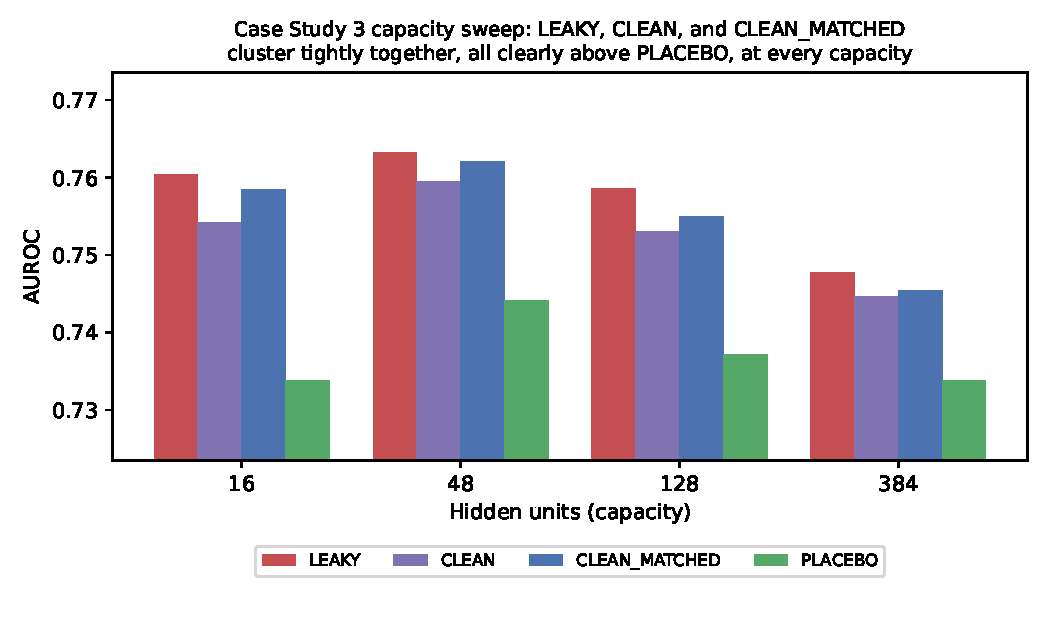
\includegraphics[width=0.75\textwidth]{figures/capacity-sweep.pdf}
\caption{Mean AUROC for LEAKY, CLEAN, CLEAN\_MATCHED, and PLACEBO across all four tested capacities. LEAKY, CLEAN, and CLEAN\_MATCHED cluster tightly together at every capacity, all clearly above PLACEBO; the gap that constitutes actual leakage severity (LEAKY vs.\ CLEAN\_MATCHED) is visually small relative to this overall separation.}
\label{fig:capacity-sweep}
\end{figure}

CLEAN\_MATCHED beats PLACEBO decisively at every capacity ($p<0.0001$,
gaps $+0.016$ to $+0.033$), confirming honest checkpoint selection is
itself strongly informative. The LEAKY$-$CLEAN\_MATCHED residual -- the
actual leakage estimate -- survives Holm-Bonferroni correction across the
four capacities at 48 and 128 units ($p=0.015$, $p=0.008$); it is
near-zero at 16 units and borderline at 384 (exact MDE $\approx 0.0038$
against an observed gap of $0.0027$: underpowered, not null). This
correction is applied within this four-capacity family only, not jointly
across every p-value reported in this section.

\textbf{Testing an alternative explanation directly.} An independent review
proposed that LEAKY's advantage might reflect ``having adaptive checkpoint
selection at all'' during a full-budget run, not fold reuse specifically,
since CLEAN\_MATCHED's full-budget retrain is a blind, fixed-epoch run
rather than an adaptively-selected one. We tested this with a fifth
condition, CLEAN\_MATCHED\_ADAPTIVE: full training budget and \emph{ongoing}
adaptive checkpoint selection during that same run -- the identical
mechanism LEAKY uses -- but selecting against the disjoint, honestly
held-out carve-out instead of the reused fold
(\texttt{code/22\_epoch\_forcing\_confound\_control.py}). If ``having adaptive
selection'' were the true driver, CLEAN\_MATCHED\_ADAPTIVE should approach
LEAKY. It does not: at capacity 128, LEAKY beats CLEAN\_MATCHED\_ADAPTIVE
by $+0.0198$ ($p<0.0001$) -- larger than the original LEAKY$-$CLEAN\_MATCHED
gap, not smaller -- and CLEAN\_MATCHED\_ADAPTIVE itself underperforms the
blind CLEAN\_MATCHED control ($-0.0164$, $p<0.0001$). At capacity 384 the
same pattern holds and is significant ($+0.0143$, $p<0.0001$), where the
original comparison was only borderline.

\textbf{How much this control can actually settle.} The honest reading is
limited by the control's own power, which we quantify directly rather
than assert. Measured on the scale that matters for this question --- how
much of honest checkpoint selection's benefit over the placebo the
control still retains, $(\text{CLEAN\_MATCHED\_ADAPTIVE} -
\text{PLACEBO})/(\text{CLEAN\_MATCHED} - \text{PLACEBO})$, computed from
\texttt{results/epoch\_forcing\_confound\_control.json} --- the control
retains only $37.3\%$ at capacity 128 ($+0.0098$ of $+0.0262$) and
$25.7\%$ at capacity 384 ($+0.0040$ of $+0.0156$). A condition that has
lost roughly two-thirds to three-quarters of the effect it was supposed
to hold constant is not a sharp instrument for adjudicating what the
remaining difference is due to. So: this test retains only
$\sim$26--37\% of honest selection's placebo-relative benefit and
therefore has limited power to adjudicate the ``any adaptive selection
helps'' alternative. Its result is directionally inconsistent with that
alternative --- LEAKY beats CLEAN\_MATCHED\_ADAPTIVE by more, not less,
than it beats CLEAN\_MATCHED --- but we do not treat this as having ruled
the alternative out.

CLEAN\_MATCHED\_ADAPTIVE's own underperformance relative to the blind
CLEAN\_MATCHED control is itself unexpected and not fully explained --
selecting against genuine, honestly held-out signal should not do worse
than blindly reusing an epoch count learned from a separate, smaller-budget
run. The most likely account, by analogy with the epoch-count mechanism
identified below for the CLEAN\_MATCHED-vs-PLACEBO anomaly, is that
adaptive selection against a small (15\%) carve-out is itself a noisy
selection signal, a different phenomenon from the fold-reuse question
this control was built to isolate. \textbf{This carve-out is also a genuine,
disclosed confound with LEAKY vs.\ CLEAN\_MATCHED\_ADAPTIVE specifically,
not just with CLEAN\_MATCHED\_ADAPTIVE's own baseline behavior}: LEAKY
selects against its full 112-sample validation fold ($560/5$), while
CLEAN\_MATCHED\_ADAPTIVE selects against only a 67-sample carve-out
($15\%$ of the $448$-sample training split) -- a $1.67\times$ difference
in selection-set size. If a smaller selection set makes
CLEAN\_MATCHED\_ADAPTIVE's own checkpoint choice noisier (which its
underperformance against blind CLEAN\_MATCHED is itself evidence for),
that same noise would inflate, not just accompany, the LEAKY-vs-CLEAN\_MATCHED\_ADAPTIVE
gap this control reports as its headline result -- so the comparison
this control is built to settle is not fully isolated from the
confound it separately flags. A cleaner version of this control would
size the carve-out to match the fold ($25\%$ of $448=112$) rather than
the $15\%$ used here; we did not rerun it at that setting, and flag this
as an open robustness gap rather than treat the current result as fully
conclusive on its own.

\textbf{A second, structurally different generative process -- with two
disclosed confounds of its own.} The sweep above draws each class from
an isotropic Gaussian (identity covariance, classes differing only in a
constant mean offset) -- a reasonable calibration device, but a
toy-model artifact is a live alternative explanation if the severity
estimate depends on that assumption rather than being a property of the
underlying leakage mechanism. We built a second generative process that
keeps the controlled, repeatable sweep design but replaces the
covariance structure: fit the real pooled within-class covariance and
mean-difference direction from the real Mistral-7B/HaluEval features
already used below, then rescale the mean difference (keeping the real,
anisotropic, correlated covariance shape exactly as observed) to hit the
same AUROC$=0.80$ calibration target via the binormal identity
(\texttt{code/27\_anisotropic\_covariance\_capacity\_sweep.py}, $n=100$ seeds, same
four capacities). Two confounds with the isotropic sweep, caught by a
fresh review, limit how cleanly this isolates covariance shape alone:
the feature dimensionality changes from 64 (isotropic) to 414 (real
features' native dimension), a $6.5\times$ change in the
dimension-to-sample ratio that itself affects checkpoint-selection
dynamics; and the realized empirical AUROC under the trained MLP is
$0.672$-$0.681$ across capacities, not the $0.753$-$0.765$ the isotropic
sweep actually achieves despite both targeting the same Bayes-optimal
$0.80$ -- the two sweeps are calibrated to the same ceiling but do not
land at the same empirical difficulty, so some of the gap difference
between them is not attributable to covariance shape alone.

With those two confounds disclosed, the pattern itself: LEAKY vs.\
CLEAN\_MATCHED is $+0.0082$ ($p=0.007$, capacity 128, vs.\ $+0.0034$
under the isotropic sweep) and $+0.0099$ ($p=0.009$, capacity 384,
vs.\ $+0.0027$, not significant, under the isotropic sweep) -- both
significant where capacity 384 previously was not. But only one of the
four capacities (128) is significance-concordant between the two
sweeps; capacity 48 goes from significant (isotropic, $p=0.015$) to not
(anisotropic, $p=0.22$), and capacity 384 goes the other way. At the two
lower capacities, LEAKY vs.\ CLEAN\_MATCHED weakens (capacity 16:
$+0.0000$, $p=0.85$; capacity 48: $+0.0016$, $p=0.22$), while
CLEAN\_MATCHED vs.\ PLACEBO becomes significant instead at those same two
capacities ($+0.0084$, $p=0.015$; $+0.0080$, $p=0.010$). Reporting all
four capacities for this comparison, not only the two where it is
significant: capacity 128 is $+0.0024$ ($p=0.45$, not significant) and
capacity 384 \emph{reverses sign} to $-0.0037$ ($p=0.11$, also not
significant) -- permuted-label checkpoint selection nominally
outperforming honest checkpoint selection at capacity 384, the same
sign anomaly the epoch-count diagnostic (Appendix A) was built to
explain and that this appendix confirms does not recur under either
corrected real-feature calibration. Some real gap is present at every
capacity under one comparison or the other, not concentrated only where
the isotropic sweep found it, but the specific capacity-by-capacity
pattern reshuffles rather than replicating cleanly. We also note that
pooling all eight synthetic LEAKY-vs-CLEAN\_MATCHED tests (both sweeps)
into one Holm-Bonferroni family, rather than treating the anisotropic
sweep as a separate robustness check the way this paper treats the
adaptive-selection control elsewhere, would leave nothing significant at
the family-wise $0.05$ level (smallest $p=0.007\times8=0.056$); we report
the anisotropic sweep's $p$-values uncorrected, in that same
robustness-check role, not as a second independent confirmation carrying
equal inferential weight to the pre-registered isotropic family. Taken
together this is evidence against the isotropic-covariance assumption
alone being responsible for the severity estimate, and does not shrink
or eliminate the gap -- but it is weaker, less clean evidence than a
simple ``replicates and is larger'' summary would suggest.

\textbf{Real-feature validation.} Feeding real Mistral-7B/HaluEval features
($n=400$, MultiHaluDet's own unmodified feature-extraction code, a 4-bit
AWQ checkpoint pinned to a fixed revision) through the same 5-fold
out-of-fold-plus-meta-learner LEAKY/CLEAN\_MATCHED/PLACEBO architecture
used in the synthetic sweep above -- not the single-fold variant an
earlier version of this test substituted, caught during review (Appendix
A) -- gives LEAKY beating CLEAN\_MATCHED by only $+0.0002$ AUROC
($p=0.56$, $n=100$ seeds) at capacity 128 and $+0.0001$ ($p=0.96$) at
capacity 384. \textbf{This comparison is not actually usable as reported: every
condition operates at AUROC $\approx0.985$ on these real features} --
the same ceiling problem Appendix A's own first correction-history entry
identifies for this paper's earlier calibration bug (``a task with no room
to fail leaves no room for a leakage bug to show inflation either''). An
absolute-AUROC-point MDE computed at a $0.80$ operating point (the
synthetic sweep's calibration target) is not comparable to an effect
measured at a $0.985$ operating point; a fresh review caught this and it
is a real, separate error from the architecture mismatch, not a
restatement of it.

\textbf{Attempted correction: calibrating the real features to the same
operating point as the synthetic sweep -- and a second, deeper problem
this attempt surfaced.} We rescaled only the between-class mean
separation of the real features (keeping every sample's own real,
unmodified within-class deviation exactly as observed -- no Gaussian
resampling, unlike the anisotropic sweep below) by the binormal-identity
factor used throughout this paper, targeting the synthetic sweep's
AUROC$=0.80$ calibration (\texttt{code/31\_real\_feature\_test\_calibrated.py}). A
further, independent review found this factor was itself computed from a
biased estimator: a permutation test (shuffling labels and recomputing
the identical plug-in formula) gives an ``achieved'' separation
($J\approx2.3$) that already exceeds the value this paper defines as
corresponding to AUROC$=0.80$ ($J=1.42$) -- pure label noise registers as
more separated than the calibration target itself, because the plug-in
Mahalanobis distance is unstable once feature dimensionality (414) is
comparable to sample size (400). We replaced this with an empirical
calibration (\texttt{code/33\_real\_feature\_test\_cv\_calibrated.py}): bisection
search over the rescaling factor, using 5-fold cross-validated,
regularized logistic regression to measure, rather than analytically
predict, the achieved AUROC at each candidate value. This gives a
rescaling factor that hits AUROC$=0.80$ by the measure used to calibrate
it ($0.795\pm0.013$, 10-seed re-check).

\textbf{A further, deeper problem: the calibration itself leaked label
information across the split it was later evaluated on.} A further
independent review found this rescaling factor -- and the diagnosis
built on it in an earlier version of this section -- rested on a
transform that centers class means on the \emph{full} labeled sample
before any train/test split exists. Because each class's per-sample
deviations sum to exactly zero over the sample used to estimate the
class means, any subsequent split mechanically forces the two halves'
leftover class-mean directions into an algebraic identity
($n_{\text{tr}}\cdot\overline{\Delta}_{\text{tr}} =
-n_{\text{te}}\cdot\overline{\Delta}_{\text{te}}$), which we verified
directly at $\alpha=0$: $\cos(\Delta\mu_{\text{train}},
\Delta\mu_{\text{test}})=-0.9999$, and a linear model fit on train and
scored on test gives AUROC $=0.06$ -- not ``zero separation,'' but
near-perfect, mechanically-induced anti-correlation. This is the exact
leakage pattern this paper's own checklist names (§5): a full-dataset,
label-dependent transform, applied before the split it is later
evaluated on -- committed by this paper's own severity-measurement
instrument.

\textbf{First fix, and a residual leak inside the fix.} We re-centered on
train indices only, applying the resulting affine map to both splits
(\texttt{code/43\_calibration\_leakage\_diagnostic.py}). That removes the
algebraic artifact: at $\alpha=0$, $\cos(\Delta\mu_{\text{train}},
\Delta\mu_{\text{test}})=0.0000\pm0.0007$ and train-fit$\to$test-eval
AUROC $=0.58\pm0.06$, not the prior draft's mechanically-guaranteed
$-0.9999$/$0.06$. \textbf{But a further independent review found this fix
incomplete in precisely the way that makes it interesting.} Estimating
the class means from train only fixes \emph{estimation}; it does not fix
\emph{application}. The transform still decided which class offset to
subtract from each point --- test points included --- by reading that
point's own label (\texttt{mask = y == cls} ranges over the whole array).
That is a residual, smaller-scale instance of the same Mechanism-1
pattern, committed by this paper's own instrument for the second time in
the same script. Its signature is visible: at $\alpha=0$, where classes
should be exactly indistinguishable, that transform still leaves a
train-fit$\to$test-eval AUROC of $0.584\pm0.059$, not chance.

\textbf{Second fix: a fully label-free calibration.} The replacement
consults no per-sample label at all. From the train indices only we
estimate the class-mean axis $u$, the midpoint $c$, and the pooled
within-class SD along $u$, $s_w$; then every row of the matrix ---
train and test alike --- is passed through the identical map
$p\mapsto\alpha p+\sqrt{1-\alpha^{2}}\,s_w\varepsilon$ on its projection
$p=\langle x-c,u\rangle$, with $\varepsilon\sim\mathcal{N}(0,1)$ drawn
independently. This shrinks the between-class separation along $u$ by
exactly $\alpha$ while preserving the marginal spread along $u$, so
difficulty is monotone in $\alpha$ and reaches chance exactly at
$\alpha=0$ --- which it does: $0.487\pm0.092$, statistically
indistinguishable from $0.5$, versus the label-conditional version's
residual $0.584$.

\textbf{A simpler label-free candidate that does not work, reported
because the negative result is load-bearing.} The obvious label-free
alternative is pure directional shrinkage toward the midpoint,
$x\mapsto x-(1-\alpha)\langle x-c,u\rangle u$, with no noise
re-injection. It consults no label --- but for any $\alpha>0$ it is an
\emph{invertible linear map}, so it cannot reduce linear separability at
all: it rescales the discriminative axis and the within-class spread
along that axis by the identical factor, leaving $d'$ unchanged. Measured
behaviour confirms this exactly: AUROC $0.993$ at $\alpha=0.2031$ where
the label-free axis-noising transform gives $0.671$. Both transforms are
retained in \texttt{code/43}'s diagnostic so this rejection is
reproducible rather than asserted.

\textbf{Re-derivation under the label-free calibration.} The alpha search
converges to $\alpha=0.3359$, achieving CV AUROC $0.7995$ against the
$0.80$ target --- and, unlike every previous version of this test, the
calibration now actually reaches its intended operating point rather than
saturating far above it.

Under the downstream 5-fold OOF-plus-meta-learner severity pipeline, the
operating point falls to $\approx0.94$-$0.95$ (LEAKY $0.9403$ at capacity
128, $0.9460$ at 384), down from the $\approx0.96$-$0.97$ the
label-conditional calibration produced and much further from the $0.985$
ceiling the original version of this test ran at --- but still above the
$0.80$ the calibration search itself achieves under plain regularized
logistic regression. The residual gap is a real, separately-documented
effect: the MLP-plus-meta-learner stack recovers discriminative structure
in directions other than the single axis the calibration operates on. A
direct severity-magnitude comparison against the synthetic sweep's $0.80$
harness therefore remains invalid by this paper's own stated principle,
and we do not make one.

At its own achieved operating point, the real-feature test now gives:
LEAKY beats CLEAN\_MATCHED by $+0.0093$ (BCa 95\% CI $[+0.0060,+0.0134]$,
capacity 128) and $+0.0077$ (CI $[+0.0050,+0.0109]$, capacity 384). Both
are strongly significant under both tests we report --- Wilcoxon
$p=7.3\times10^{-7}$ and $1.4\times10^{-5}$, paired permutation
$p<0.0001$ at both capacities --- and, importantly, the two tests now
agree, which they did not under the previous calibration (see the tie
disclosure below). CLEAN\_MATCHED beats PLACEBO decisively at both
capacities ($+0.0151$, $p=9.4\times10^{-7}$; $+0.0091$,
$p=1.0\times10^{-5}$), again confirming substantial real,
non-leakage-driven signal in honest adaptive checkpoint selection on real
features.

\textbf{Tie disclosure for these Wilcoxon tests.} The paired differences
here contain many tied absolute values --- $33$ of $100$ at capacity 128
and $40$ of $100$ at capacity 384 (plus $1$ and $2$ exact zeros
respectively), because AUROC on a $80$-sample test split takes discrete
values. The Wilcoxon signed-rank statistic degrades under ties, so we
report the paired sign-flip permutation test alongside it throughout
(\texttt{code/44}); here both give the same verdict. This matters because
under the \emph{superseded} label-conditional calibration the tie counts
were substantially worse ($49$ and $60$ of $100$) and the two tests
disagreed by an order of magnitude in $p$ (Wilcoxon $p=0.00064$ versus
permutation $p=0.0025$ at capacity 128) --- a fact the previous version
of this section quoted the Wilcoxon $p$ without disclosing.

\textbf{A fidelity extension: the checkpoint-selection-only harness
understates what the audited trainer actually does.} Everything above
ports only MultiHaluDet's final ``keep the best-val-AUROC checkpoint''
decision. Its real trainer also steps a \texttt{ReduceLROnPlateau}
scheduler on that same fold's AUROC every epoch and ties early stopping
to the same signal --- a continuous reactive coupling, not a single
argmax. Porting that mechanic in, with a control that keeps the same
scheduler and early-stopping mechanic but feeds it a genuinely disjoint
carve-out (\texttt{code/49}), gives LEAKY beating that control by
$+0.0221$ (BCa 95\% CI $[+0.0159,+0.0292]$, Wilcoxon
$p=1.9\times10^{-9}$, permutation $p<0.0001$, $n=100$ seeds, capacity
128) --- about $2.4\times$ the checkpoint-selection-only harness's
$+0.0093$ on the same features under the same calibration. Appendix A
(issue 12) documents four sequential control-construction bugs this
extension needed fixing for, and reports the factorial $2\times2$
ablation separating its two most recent corrections, whose interaction
turns out to be another instance of §5's operating-point relationship.

This paper's primary severity estimate for
Mechanism 3 still rests on the two synthetic sweeps, which generate
fresh samples from a fully-specified generative process each seed rather
than rescaling a small, fixed real sample, and so share neither the
analytic-bias nor the split-leakage problem found here.

A separate FP16-vs-AWQ control on the same 50
samples finds identical AUROC (0.9600 both) at a single point estimate;
a resampled version (Appendix A) gives a 95\% CI of $[-0.061, +0.080]$,
consistent with no quantization confound rather than a demonstration
that rules one out at the resolution this severity estimate needs.
Appendix A documents the full progression of this test -- the original
architecture mismatch, the ceiling-effect error the ``corrected'' version
still had, the biased calibration factor a further review caught, the
split-crossing leakage that same correction's own instrument turned out
to commit, and the properly-verified operating-point mismatch that
survives the fix -- along with a further robustness check (a
resampled-effect-size reanalysis of the FP16-vs-AWQ control).

\textbf{A pre-registered decision rule whose verdict depends on which version
of the test is asked.} Before running the sweep, we pre-registered a
rule classifying each capacity as \texttt{GENUINE\_LEAK\_CONFIRMED},
\texttt{CONFOUND\_CONFIRMED\_NO\_REAL\_LEAK}, or \texttt{MIXED} from the placebo-relative
gaps. We initially reported this branch as structurally unreachable, on
the basis that leaky\_minus\_placebo is significant at $p<10^{-8}$ ``in
every version of this experiment'' -- this was wrong, caught by the same
review that caught the ceiling-effect error above. Applying the rule to
every version actually run: the isotropic synthetic sweep returns
\texttt{MIXED} at all four capacities; the anisotropic sweep returns
\texttt{MIXED} at three and \texttt{GENUINE\_LEAK\_CONFIRMED} at one (capacity 128); the
ceiling-confounded real-feature test returns \texttt{CONFOUND\_CONFIRMED\_NO\_REAL\_LEAK}
at both tested capacities; the biased-calibration, the
leak-contaminated bias-corrected, and the (superseded) label-conditional
train-only-centered real-feature tests all return \texttt{MIXED} at both
capacities; and the current, label-free-calibrated real-feature test
returns \texttt{GENUINE\_LEAK\_CONFIRMED} at both capacities. The rule is
therefore reachable in every
direction -- what it is not, is \emph{stable}: the same underlying mechanism
produces all three verdicts depending on generative process,
calibration, and capacity. We flag this bluntly, including the fact that
the verdict moved in the \emph{favourable} direction for our own
hypothesis when the calibration was corrected: that is precisely the
circumstance in which a single pre-registered rule's output should be
trusted least, and it is why this paper's severity claims rest on effect
sizes with intervals rather than on the rule's label. We read this as reinforcing, not undermining,
this paper's central methodological point: a single pre-registered
decision rule, however principled, is not a substitute for reporting the
full distribution of outcomes across every control run, and a reader
should not take ``pre-registered'' as license to trust one capacity's
classification without checking the others; Appendix A documents the
full analysis.

\textbf{Bottom line.} The mechanism itself -- checkpoint choice as a function
of the reused fold's own labels -- is unambiguous and code-verified. Its
quantified severity, once budget- and seed-matched, is small ($+0.0009$
to $+0.0034$ AUROC on the synthetic sweep) and significant at most but not
all tested capacities. The LEAKY-vs-CLEAN\_MATCHED\_ADAPTIVE gap is larger
and more significant still, but -- as disclosed above -- that widened gap
is at least partly confounded by CLEAN\_MATCHED\_ADAPTIVE's own
underperformance relative to blind CLEAN\_MATCHED, itself most plausibly a
symptom of the smaller ($15\%$) carve-out being a noisier selection
signal rather than confirmation that fold-reuse leakage is larger than
the primary estimate; we do not treat this control as straightforwardly
strengthening the headline severity number, only as failing to support
the alternative ``any adaptive selection helps'' explanation it was built
to rule out. Severity is again small (if anything, more
strongly significant, though with a reshuffled rather than uniformly stronger
capacity pattern -- see Appendix A) under a second generative process
replacing the isotropic calibration with a real, anisotropic covariance
structure. A real-feature validation attempt went through four further
rounds of correction (an architecture-mismatch fix, a
biased-calibration-factor fix, a fix to a split-crossing leakage bug in
that very correction's own centering step, and then a fix to a residual
label-conditional step inside \emph{that} fix) before reaching a
trustworthy account: even fully leak-free, it cannot be brought onto the
synthetic sweep's $0.80$ operating point under the downstream harness
(it runs at $\approx0.94$-$0.95$), because the real feature set's
discriminative content genuinely includes structure a single-axis
calibration cannot touch -- but at its own achieved
operating point, the test gives a small, strongly significant,
BCa-confidence-bounded severity estimate ($+0.0077$ to $+0.0093$ AUROC,
permutation $p<0.0001$ at both capacities)
directionally consistent with the synthetic sweeps. This paper's primary
severity estimate for Mechanism 3 still rests on the two synthetic
sweeps, which share neither the operating-point nor the leakage problem
found here. This also does
not settle MultiHaluDet's own 98.55\% AUROC's exact inflation: their real
architecture (6 transformer layers, multi-scale, heavy augmentation) is
considerably more expressive than this reconstruction. Getting this
diagnosis right required tracing each correction to its actual source
rather than accepting a partially-improved number at face value --
including, in the end, tracing a bug in the correction script itself;
Appendix A documents that process in full.

\subsection{Case Study 4 (severity $+0.0054$ AUROC, CI $[+0.0032,+0.0100]$): Test-set-driven best-layer selection — quantized-LLM paper}

[See \texttt{draft/case\_study\_quantized\_llm\_paper.md} for full detail, including
literal code excerpts.]

``Hallucination Is Linearly Decodable from Mid-Layer Hidden States in
Quantized LLMs'' (arXiv 2606.02628; repo
\texttt{github.com/Ezharjan/HallucinationPatternDetection}, pinned at commit
\texttt{ea0b9678}) reports AUROC up to 1.000. Its per-layer probe training
(\texttt{src/detection/probes.py::train\_probe}) uses a clean single 70/10/20
train/val/test split, genuinely free of Case Studies 1-3's exact
patterns. But \texttt{src/detection/saplma.py::saplma\_probe\_per\_layer} selects a
\texttt{best\_layer} by the argmax, over ~30 layers, of each layer's \textbf{test-set}
AUROC, then reports that same test-set number as the headline result,
with no correction for having tried ~30 hypotheses against the one test
set. This is the classical ``winner's curse'' of multiple-hypothesis
selection using the exact metric later reported.

We initially believed re-quantifying this mechanism's severity would
require their exact quantized checkpoint and dataset re-run from
scratch; a fresh review found this unnecessary. Their repo ships
per-layer, per-seed AUROC arrays for all 24 model/dataset/probe-type
combinations tested (\texttt{code/external/HallucinationPatternDetection/results/probes/*.json},
33 layers, 3 seeds each). For each combination
(\texttt{code/45\_case\_study\_4\_winners\_curse.py}), each of the 3 seeds is
held out in turn; the best layer is selected using \emph{only} the other
two seeds, the naive baseline is the selection-set mean at that selected
layer, and the honest estimate is the held-out seed's AUROC at that same
layer. Their difference, averaged over the three rotations, is the
winner's-curse estimate.

\textbf{Correction (a later independent review).} An earlier version of
this script took the naive baseline from the repo's own reported
\texttt{best\_auroc}, which is a max over \emph{all three} seeds --
including the seed then used as ``held-out.'' Whenever the leave-one-out
argmax happened to coincide with the full-sample argmax (7 of 24 cells),
the two sides of the subtraction were arithmetically forced to be equal
and the estimate was pinned at exactly $0.0000$ regardless of the true
effect. Under the corrected, genuinely leave-one-seed-out protocol the
estimate is mean $+0.0054$ AUROC across all 24 combinations (BCa 95\% CI
$[+0.0032,+0.0100]$, Wilcoxon $p=0.00017$; max $+0.0347$), up from the
$+0.0047$ (max $+0.0288$) the flawed estimator reported. This section
previously carried no CI or significance test at all, unlike every other
severity estimate in this paper; that is fixed here.

\textbf{Ceiling composition of the 24 cells.} These cells are not
comparable to each other, and reporting only their pooled mean hides
that. In $12$ of $24$ the \emph{selected} layer already sits at AUROC
$\geq0.975$ (all six \texttt{halueval\_qa} cells and all six
\texttt{synthetic} cells), leaving almost no headroom for a selection
effect to be visible; the remaining $12$ (\texttt{fever},
\texttt{truthfulqa}) are genuinely non-saturated. Reported separately:
ceiling-saturated $+0.0042$ (CI $[+0.0029,+0.0057]$); non-saturated
$+0.0065$ (CI $[+0.0023,+0.0152]$, $p=0.047$). By dataset:
\texttt{fever} $+0.0124$, \texttt{halueval\_qa} $+0.0052$,
\texttt{synthetic} $+0.0033$, \texttt{truthfulqa} $+0.0007$. Under a
stricter saturation reading (every layer, not just the selected one,
above $0.975$ -- true for the six \texttt{halueval\_qa} cells) the split
is $+0.0052$ (6 cells) versus $+0.0054$ (18 cells). The mechanism's
severity is small on every slicing, and larger where there is room for
it to show, exactly as the operating-point relationship in §5 predicts.

\subsection{Mechanism 5 (found while auditing Case Study 3's own repository): Test-set-driven operating-point selection — MultiHaluDet}

A fresh, independent review found a fifth, structurally distinct
leakage mechanism sitting in the exact file this paper already audits
for Mechanism 3. \texttt{MultiHaluDet/run\_pipeline.py::stage\_4\_ensemble} calls
\texttt{find\_best\_thresholds(probs, y\_test)} (\texttt{src/utils/metrics.py}), which
sweeps 81 candidate F1 thresholds and the ROC-optimal (Youden) threshold
\emph{directly against the test labels}, then reports every threshold-dependent
metric -- F1, accuracy, Matthews correlation, Cohen's $\kappa$, balanced
accuracy, and the ECE computed from those predictions -- at that
test-label-selected threshold. AUROC is threshold-free and unaffected by
this specific bug, but every other headline number MultiHaluDet reports
is test-set-optimized operating-point selection: the choice of \emph{where to
draw the decision boundary} uses the same labels the boundary is then
scored against. This is structurally distinct from Mechanisms 1-4, which
all concern \emph{which feature, checkpoint, or layer} to use -- this one
concerns \emph{which threshold to report at}, given a fixed, already-chosen
model.

We quantified this severity using the same isotropic-Gaussian calibration
this paper's other severity estimates already rely on (binormal identity,
Bayes-optimal AUROC target), with a simple logistic-regression classifier
in place of the full SweepMLP-plus-meta-learner architecture (threshold-selection
leakage does not depend on which classifier produced the probabilities,
so a simpler classifier keeps this demonstration self-contained;
\texttt{code/46\_mechanism5\_threshold\_selection.py}). \textbf{Correction:}
an earlier version of this synthetic generator itself committed the exact
calibration-inversion class of error Lesson 5a (Appendix A) already
documents finding once elsewhere in this paper's own tooling -- the
class-mean offset used the full separation rather than half of it on each
side, silently quadrupling the realized Fisher $J$ relative to the labeled
operating point. This was caught by a subsequent independent review and
fixed (verified via a dedicated, non-tautological calibration guardrail,
\texttt{code/sanity\_checks.py}, now mandatory before any synthetic
generator in this project returns data). Comparing a threshold
selected on the test labels (\texttt{find\_best\_thresholds}, verbatim ported from
MultiHaluDet's own code) against a threshold selected on an independent
validation split never touching the test labels, across five operating
points spanning this paper's other severity estimates, under the
corrected calibration: F1 gaps ranging from $+0.0212$ ($0.985$,
MultiHaluDet's own reported regime) to $+0.0338$ (AUROC target $0.80$,
the largest of the five points, with no clean monotonic trend across
operating points: $0.70{\to}0.0228$, $0.80{\to}0.0338$, $0.90{\to}0.0311$,
$0.95{\to}0.0233$, $0.985{\to}0.0212$), all significant at $p<10^{-31}$
over $200$ seeds (BCa 95\% CIs excluding zero throughout); accuracy gaps
of comparable magnitude ($+0.0215$ to $+0.0457$).

\textbf{A necessary caveat on comparing this to Mechanism 3: these are not
the same metric, and the comparison is not like-for-like.} AUROC is
threshold-free by construction, so test-set threshold selection has
\emph{exactly zero} effect on it -- Mechanism 5's severity on the one
metric it shares with Mechanism 3 is not small but precisely nil. The F1
gap reported above is also structurally guaranteed non-negative: the LEAKY
threshold is chosen by an argmax over the very same grid the test F1 is
then scored on, so it cannot do worse than any other threshold drawn from
that grid, including HONEST's. An earlier draft of this section compared
these F1/accuracy gaps directly against Mechanism 3's AUROC gaps and
described Mechanism 5 as ``an order of magnitude more severe'' -- that
comparison conflated two different metrics measuring two different
things and has been removed. The honest statement is narrower: Mechanism
5 leaves the pipeline's reported AUROC entirely unaffected, but materially
inflates every threshold-dependent metric (F1, accuracy, MCC, Cohen's
$\kappa$, and any ECE computed from those threshold-derived predictions)
that MultiHaluDet also reports at that same selected threshold -- a
distinct, real leak in its own right, not a directly rankable ``more or
less severe than Mechanism 3.''

\section{What Actually Governs Severity: Candidate Count and Operating Point}
\label{sec:governs}

The five mechanisms above are structurally distinct, and identifying them
is this paper's most durable contribution. But once each is measured
against matched controls, the striking result is how \emph{little} their
severities differ from one another --- and how much they differ across
conditions that have nothing to do with which mechanism is responsible.
This section states that finding directly; the sweep behind it is
reported cell-by-cell in Appendix A.

\textbf{The measured severities cluster.} Every mechanism in this paper
with a code-verified AUROC-scale estimate lands in a narrow band. Under
randomized splits, Mechanism 2's selection-specific component is
$+0.027$ (SD $0.021$). Mechanism 3's checkpoint-selection severity is
$+0.0009$ to $+0.0034$ on the isotropic synthetic sweep, $+0.0000$ to
$+0.0099$ on the anisotropic sweep, and $+0.0077$ to $+0.0093$ on the
real-feature harness; extending it to model the audited trainer's full
LR-scheduler-plus-early-stopping coupling raises it to $+0.0221$
(Appendix A, issue 12). Mechanism 4's is $+0.0054$ across 24 published
cells ($+0.0065$ on the non-saturated half). Mechanism 5's effect on
AUROC is exactly zero by construction, while its effect on the
threshold-dependent metrics the same pipeline reports is $+0.021$ to
$+0.034$ in F1. That is a spread of roughly $0.000$ to $0.027$ AUROC
across four structurally unrelated leakage surfaces in two independent
published pipelines --- all small, and none separated from the others by
anything like the margin an ``it depends which leak you have'' framing
would need.

\textbf{Two continuous quantities move severity far more than mechanism
identity does.} \texttt{code/47\_selection\_multiplicity\_sweep.py} varies,
one at a time, the number of candidates selected among ($K$), the
selection-set size ($n_{\text{val}}$), and the model's operating point
(the calibrated Bayes-optimal AUROC), holding the leakage mechanism
itself fixed:

\begin{itemize}
\item \textbf{Candidate count.} Sweeping $K\in\{1,\ldots,225\}$ moves the
  gap monotonically from $+0.0000$ to $+0.0052$, well described by
  $\text{gap}=a+b\ln K$ ($R^2=0.970$). Note this is an empirical
  logarithmic regularity, \emph{not} a confirmation of the
  $\sigma_{\text{val}}\sqrt{2\ln K}$ extreme-value form, which is
  falsified on this data once fit as stated (Appendix A).
\item \textbf{Operating point.} This is the largest effect anywhere in
  this paper. Holding the mechanism, $K$, and $n_{\text{val}}$ fixed and
  varying only the calibrated difficulty of the task, the gap falls from
  $+0.0093$ at AUROC$_0=0.70$ to $+0.0037$/$+0.0011$/$+0.0007$ at
  $0.80$/$0.90$/$0.95$ and to $+0.0002$ at $0.985$ --- a
  \textbf{$48.6\times$ decline}, one and a half orders of magnitude,
  driven by nothing but where on the difficulty curve the pipeline
  operates.
\item \textbf{Selection-set size.} Directionally consistent with the
  winner's-curse account (largest gaps at small $n_{\text{val}}$) but
  \emph{not} cleanly monotone across the three points tested: $+0.0026$
  ($n_{\text{val}}\approx56$, not significant), $+0.0036$
  ($\approx112$), $+0.0005$ ($\approx448$). We report this as the
  weakest of the three relationships.
\end{itemize}

\textbf{Why this matters practically.} The operating-point relationship
explains, without appeal to mechanism identity, why several severity
estimates in this paper come out near zero: they were measured on tasks
already running at AUROC $\geq0.98$, where there is almost no headroom
for selection to inflate anything. That includes the 12 ceiling-saturated
cells of Case Study 4 ($+0.0042$ versus $+0.0065$ on the non-saturated
half), MultiHaluDet's own $0.985$ regime, and this paper's own
real-feature harness before it was recalibrated. A reader auditing a
pipeline should therefore ask \emph{how many candidates were tried} and
\emph{where on the difficulty curve the reported number sits}, not
primarily \emph{which of the five mechanisms} is present --- while still
using the mechanism taxonomy to know where to look.

\textbf{What this does not establish.} These sweeps vary one quantity at
a time within a single synthetic harness holding the mechanism fixed;
they do not constitute a matched head-to-head across all five mechanisms
at common $(K, n_{\text{val}}, \text{AUROC}_0)$, which would be needed to
test whether mechanism identity explains any \emph{residual} variance
once these three are controlled. We do not claim it explains none. That
experiment is the obvious next step and is not run here.

\section{A Checklist for This Literature}

[Full version in \texttt{draft/leakage\_checklist.md}.] Five questions correspond
to the five mechanisms above:

\begin{enumerate}
\item Is any feature computed by fitting something on the full dataset's
   labels before an outer CV loop treats part of that dataset as held out?
\item Inside a CV fold, is a ``best'' checkpoint/epoch chosen using the same
   fold whose features/predictions get reused downstream as clean OOF
   output?
\item Is a ``best'' layer/config selected by the argmax of a metric computed
   on the same test set later reported as the headline number, across
   many candidates, with no correction?
\item Was a hyperparameter chosen by maximizing a cross-validated metric,
   with that same CV number then reported as performance, with no
   further genuinely held-out check?
\item Was a decision threshold or other operating point chosen by
   optimizing a metric on the test labels themselves, with that same
   test set then used to report the metric at that threshold?
\end{enumerate}

\textbf{We tried to automate this checklist; the attempt itself is informative.}
We built a regex-based scanner for the original four patterns (Mechanism
5 was found after this scanner was built and is not yet covered by it)
and ran it against 7
repositories total: the two already-audited case studies (MultiHaluDet,
HallucinationPatternDetection), to test whether it catches known bugs,
plus 5 additional, not-previously-examined, externally-found
hidden-state-probing repositories, to test its false-positive rate on
presumed-clean pipelines (\texttt{code/04\_leakage\_linter.py},
\texttt{results/leakage\_linter\_report.json}). This is a heuristic line-matcher,
not a validated static analyzer; every flag was manually read and
classified before being treated as a finding.

The scanner produced 7 raw hits, concentrated in 2 repos, and manual
reading showed all 7 are false positives: 3 flag
\texttt{HallucinationPatternDetection}'s \texttt{embed\_viz.py} for ``fit-then-score'' --
these are t-SNE/UMAP/PCA calls used only for plotting; 4 flag
\texttt{haloscope}'s layer/threshold selection -- reading the code shows
selection correctly uses a separate validation split, the opposite of
leakage, and a positive data point for that NeurIPS 2024 pipeline. More
tellingly, the scanner missed both known true positives in this corpus.
\textbf{Both misses have specific, identifiable causes in this scanner's
own construction, and we name them rather than generalizing from them.}
(i) Case Study 3's selection site (\texttt{trainer.py}, lines 137-144)
binds \texttt{best\_auc}/\texttt{best\_model}; the scanner's
\texttt{CHECKPOINT\_KEYWORDS} list (\texttt{code/04}, line 55) contains only
\texttt{best\_epoch}, \texttt{best\_checkpoint} and \texttt{checkpoint}. This
is a plain keyword-list gap -- and a telling one, since we had already
read those exact two token names while manually diagnosing the bug and
still did not add them. (ii) Case Study 4's selection site
(\texttt{saplma.py}, lines 32-41) \emph{is} matched by
\texttt{ARGMAX\_KEYWORDS}, which already contains \texttt{best\_layer}; what
fails is the scanner's design choice to require an argmax token and a
\texttt{test}-named variable \emph{on the same line}, and, before that, in
the same file. That file contains no \texttt{test}-named identifier
anywhere -- the test split lives one call away, in
\texttt{probes.py::train\_layerwise\_probes} -- so a same-file, same-line
conjunction cannot fire on it however the keyword lists are extended.
Zero true positives among the 5 newly-scanned repos, two false negatives
on the two known positives, seven-for-seven false positives on its raw
hits: this particular scanner does not work. We deliberately do not read
that as evidence that the leakage class is inherently resistant to
static detection. Cause (i) would be fixed by a longer keyword list, and
cause (ii) points at a specific, tractable design requirement -- the
argmax and the test-derived metric must be connected across statements
and across function boundaries, i.e.\ by a dataflow analysis rather than
line matching. What this exercise establishes is narrower and more
useful: \emph{line-level regex matching} is the wrong tool here, because
every one of these mechanisms is a relationship between a selection
statement and the provenance of the quantity it selects on, and that
relationship is routinely split across lines, functions, and files.

This is a prevalence statement about 2 of 7 repos, not a representative
sample -- all 7 were found via targeted search for exactly this failure
class, not a random or exhaustive sample of the field (HaRP and GUARDIAN,
this paper's own pipelines and the source of Case Studies 1-2, were never
run through the scanner at all -- they sit entirely outside this count).
The true population-level prevalence of any
of these five mechanisms remains unknown and is not estimated by this
count. We report the negative automation result because the same
variable-naming and control-flow subtlety that makes this leakage easy to
introduce by accident also defeats line-level pattern-matching, in both
directions -- not because we have shown that a better-designed static
analyzer would also fail. Building and validating that analyzer is
follow-on work this paper does not do.

\section{Discussion}

\textbf{Data and code availability.} All code, cached result JSONs, and the
paper source are included in the anonymized supplementary material for
double-blind review, and will be released as a public GitHub repository
under the authors' names upon publication. Case Studies 2, 3 and 4 are
reproducible from what ships with this paper: pinned third-party commits,
our audit scripts, the resulting JSON logs, and --- for Case Study 2,
whose original 171\,MB hidden-state cache is too large to ship --- a
$\sim$1\,MB derived artifact of per-layer probe scores and fold
assignments plus a replay script (\texttt{code/51}) that recomputes and
asserts every reported number from it. \textbf{Case Study 1 is the
exception and we state it plainly: no script, log, or data file
supporting its $+0.19$ figure is included here, and that number should
not be treated as verified by this artifact} (§4). The regex
linter in §5 is included in full and is, per its own results, a confirmed
non-detector on this corpus (0 true positives, 2 false negatives on the
corpus's own known bugs) -- included for transparency, not as a working
tool a reader should rely on today.

\textbf{Scope note.} This paper makes no inference-economy claim. It is an
evaluation-protocol audit, not an inference-time method; fixing any of
the five leakage mechanisms makes no claimed difference to deployment
cost. The paper's value is entirely in correcting reported detection
metrics.

\textbf{Severity numbers matter operationally, even though we do not quantify
deployment cost here --- and the honest headline is that they are small.}
A detector deployed at a reported AUROC above its true value will, at a
fixed threshold, pass more hallucinations to production and flag more
correct outputs for unnecessary review than promised. But the
code-verified inflations this paper measures are on the order of $0.002$
to $0.027$ AUROC, not the tens of points an earlier framing of this work
implied. Practitioners should read this as: these mechanisms are real,
worth fixing because they are cheap to fix and because they corrupt
comparisons between methods, but not as an argument that the subfield's
reported numbers are broadly wrong by large margins. We lack
deployment-volume and review-cost data for any audited system, so we do
not attempt a cost estimate. Where large gaps \emph{do} appear
(Mechanism 5's $+0.021$ to $+0.034$ on F1 and accuracy), they are on
threshold-dependent metrics, not AUROC, and are not directly comparable
to the AUROC-scale numbers.

\textbf{This audit's central lesson recurs in related, independently-conducted
work} examining hidden-state signals and benchmark severity estimates
in adjacent areas of LLM evaluation, none sharing a leakage mechanism
with the four case studies here: an initially plausible signal or
benchmark result substantially weakens or changes character once a
specific confound is directly tested, rather than merely acknowledged as
possible. This paper shares that discipline: a claimed severity or
signal is not established until the confounds that could produce it for
free have been named and tested, not merely acknowledged as possible.

\textbf{Limitations.} \emph{(1) Case Study 1 is not re-verifiable from
this artifact} --- no supporting script, log, or data ships with the
paper, and its $+0.19$ figure is excluded from every quantitative claim
here. \emph{(2) The central severity relationship (§5) is measured
one-quantity-at-a-time in a single synthetic harness with the mechanism
held fixed.} It shows that $K$ and the operating point move severity a
great deal; it does not show that mechanism identity explains \emph{no}
residual variance once those are controlled. A matched
$(K, n_{\text{val}}, \text{AUROC}_0)$ head-to-head across all five
mechanisms in one harness would test that directly and is not run here.
\emph{(3) The extreme-value-theory account of $K$-scaling is falsified
in this harness} once fit as stated (Appendix A); we report an empirical
logarithmic regularity instead and do not have a mechanistic
explanation for it. \emph{(4) The alternative-confound control for
Mechanism 3 retains only $\sim$26--37\% of honest selection's
placebo-relative benefit} and therefore has limited power (§4.3).
\emph{(5)} We could not re-run either external paper's full
7B-scale pipeline within this paper's compute budget, so Case Studies 3
and 4's severity for the \emph{actual published numbers} remain open
questions; our reconstruction of Case Study 3 supports a small, positive
estimate at 2 of 4 tested capacities, and MultiHaluDet's actual
architecture (6 transformer layers, multi-scale, heavy augmentation) is
more expressive still, so this should not be over-read in either
direction for their pipeline. The real-feature test (\S4.3) is also
single-dataset, single-language ($n=400$ HaluEval English \texttt{qa\_samples}
only), despite MultiHaluDet's own contribution being explicitly
multilingual; and even leak-free, no calibration of this feature set's
between-class mean, at any strength, brings it onto the synthetic
sweep's exact $0.80$ operating point, because a real portion of its
discriminability lives in within-class structure the calibration method
cannot touch -- so its severity estimate, while now trustworthy, is
reported at its own ($\approx0.94$-$0.95$) operating point rather than
the synthetic sweep's, and the two are not numerically comparable.
Whether the synthetic severity estimate transfers to real hidden states
at the \emph{same} operating point -- on this dataset, non-English
datasets, or larger ones -- remains untested rather than confirmed or
excluded, and would need a different validation strategy than
mean-only rescaling to test at this sample size and dimensionality.

\section{Conclusion}

Five distinct label-information-leakage mechanisms recur across
hidden-state hallucination-detection pipelines, including our own. Three
of the five are verified directly against pinned commits of externally
published code. That taxonomy is this paper's most durable contribution,
and we expect it to outlast every number in it.

\textbf{The severities, however, do not differ sharply --- and an earlier
version of this work was wrong to say they did.} Measured against matched
controls, every mechanism here with a code-verified AUROC-scale estimate
lands between roughly $0.000$ and $0.027$ AUROC: Mechanism 2's
selection-specific component $+0.027$ (SD $0.021$, $p=0.009$) under
randomized splits; Mechanism 3's checkpoint-selection severity $+0.0009$
to $+0.0034$ on the isotropic synthetic sweep, significant at 2 of 4
tested capacities; Mechanism 4's $+0.0054$ (BCa 95\% CI
$[+0.0032,+0.0100]$) across 24 published result files; Mechanism 5's
effect on AUROC exactly zero by construction. Case Study 1's much larger
$+0.19$ figure is reported from prior work and is \emph{not}
re-verifiable from this artifact, so we exclude it from that comparison
rather than let it carry the claim.

\textbf{What severity does track is continuous and
mechanism-independent.} Holding the leakage mechanism fixed and varying
only the number of candidates selected among moves the gap
monotonically, well fit by $a+b\ln K$ ($R^2=0.970$); varying only the
operating point moves it by $48.6\times$, from $+0.0093$ at
AUROC$_0=0.70$ to $+0.0002$ at $0.985$ (§5). Both effects are larger
than any difference we measure between mechanisms. We report a
correction here as well: an earlier draft described the $K$-scaling as
confirming the extreme-value-theory prediction
$c\,\sigma_{\text{val}}\sqrt{2\ln K}$ at $R^2=0.756$. That fit held
$\sigma_{\text{val}}$ fixed at its cross-cell mean. Refit as the theory
states it, with each cell's own measured $\sigma_{\text{val}}$ --- which
varies $2.66\times$ across the sweep and moves \emph{opposite} to the gap
--- the EVT form gives $R^2=-0.399$, worse than predicting the mean. The
$K$-scaling is real; the extreme-value functional form for it is not
supported by this data (Appendix A).

Mechanism 5 remains a clear case that a pipeline can be simultaneously
clean on one reported metric and leaking on another: it leaves AUROC
exactly unaffected while producing F1/accuracy gaps of $+0.021$ to
$+0.034$ that are large and highly significant on their own terms,
though not directly comparable in magnitude to the AUROC-scale numbers.
And the difficulty of establishing any of these numbers --- needing
calibration, budget-matching, seed-matching, an alternative-confound
test, and a leak-free measurement instrument all to hold at once --- is
the strongest argument in this paper for the checklist we provide, more
so than any single mechanism in isolation.

The checklist lets researchers and reviewers in this fast-growing
subfield ask precise, mechanism-specific questions of a pipeline's
evaluation protocol, replacing ``did you use cross-validation correctly''
as a single, undifferentiated concern.

The automated-scanner exercise (§5) covers seven repositories in total:
two already-confirmed positive case studies (§4.3-4.4, MultiHaluDet and
HallucinationPatternDetection) and five additional, not-previously-examined
repositories, which surfaced no new confirmed positives -- too small a
sample to support any claim about how common these five mechanisms are
across the wider literature, and we do not make one. (Case Studies 1-2,
HaRP and GUARDIAN, were manually audited and are not part of this count
at all.) A pre-registered audit applying
this checklist to a fixed,
defined sample of 15-20 externally published probing papers, selected
before any of them are examined, is planned as follow-on work; that
protocol is already drafted.

\section{Appendix A: Correction History and Robustness Checks for Case Study 3 (MultiHaluDet)}

\textbf{This appendix documents how the Case Study 3 result in §4.3 was
reached, and additional robustness checks omitted from the main text for
length.} §4.3 states the result directly; nothing below is required to
verify it.

\textbf{TL;DR.} Thirteen issues were found and fixed via iterative review while
deriving this case study's severity estimate (full table below). In
order: (1) an uncalibrated
synthetic sweep saturated at AUROC=1.0; (2) the calibration formula
itself was inverted; (3) LEAKY/CLEAN were not budget- or seed-matched;
(4) the real-feature test's architecture did not match the synthetic
sweep's (single-fold MLP vs. the intended 5-fold OOF+meta-learner);
(5) the ``corrected architecture'' version still ran at a saturated
operating point (AUROC$\approx0.985$); (6) the rescaling factor used to
fix (5) was itself computed from a biased, noise-inflated estimator;
(7) a permutation-null number was misattributed to the wrong check;
(8) \textbf{the calibration transform itself leaked label information across
the split it was later evaluated on} (full-sample class-mean centering
before the split) -- this is the load-bearing finding of this appendix,
and the reason this paper's own severity-measurement instrument is used
as a worked example of Mechanism 1 in §4.3; (9) fixing (8) left the
operating-point mismatch from (5) unresolved; (10) the fidelity extension
modelling MultiHaluDet's actual LR-scheduler and early-stopping behaviour
went through two sequential control-construction bugs of its own; (11)
two of this paper's synthetic generators silently realized $4\times$ the
intended Fisher $J$; (12) the fidelity extension's early-stopping
patience was set to the LR scheduler's $3$ rather than the audited
repo's own $15$; and (13) \textbf{the fix for (8) was itself still
label-conditional} --- it fixed which samples the class means were
\emph{estimated} from but not which label decided how each point was
\emph{shifted} --- replaced with a fully label-free calibration that
reaches chance exactly at zero separation, and which, for the first time
in this test's history, reaches its intended $0.80$ operating point
instead of saturating.

\textbf{The numbers that survive all thirteen and are the ones §4.3
actually reports} are stated in §4.3 and in items 9, 12 and 13 of the
table below. Two structural points about them: the two synthetic sweeps
(isotropic, anisotropic) remain the paper's primary severity estimate
for this mechanism, since they share neither the architecture-mismatch
(4) nor the split-leakage (8) problem the real-feature test needed fixing
for; and the fidelity extension's move from $+0.0111$ to $+0.0221$ is
\emph{not} attributed to either of (12) or (13) alone --- a factorial
$2\times2$ ablation (item 12) shows the patience correction's sign flips
with the operating point, which is itself the relationship §5 documents.

\textbf{Correction table.} Each row is one issue found by iterative
review while deriving §4.3's severity estimate; full derivations live in
the cited script/result files, not below.

\begin{description}
\item[1.] Uncalibrated sweep saturated at AUROC$=1.0$. \textit{Fix:}
  calibrate via $\text{AUROC}=\Phi(\sqrt{J/2})$.
\item[2.] Calibration formula was inverted ($\Phi(\sqrt J/2)$, the
  accuracy identity, not AUROC). \textit{Fix:} corrected inversion,
  $J=2\Phi^{-1}(0.80)^2=1.417$ $\rightarrow$ verified
  $\Phi(\sqrt{J/2})=0.800$.
\item[3.] LEAKY/CLEAN not budget- or seed-matched (CLEAN's ES carve-out
  $\approx$15\% less data; matched retrain used a different seed).
  \textit{Fix:} match both $\rightarrow$ result now stated in §4.3.
\item[4.] Real-feature test's architecture didn't match the synthetic
  sweep's (single-fold MLP vs. intended 5-fold OOF+meta-learner).
  \textit{Fix:} rerun with the actual architecture (\texttt{code/25})
  $\rightarrow$ $+0.0002$ ($p=0.56$, cap. 128), not significant.
\item[5.] ``Corrected architecture'' still ran at a ceiling operating
  point (AUROC$\approx0.985$), making its MDE incomparable to the
  synthetic sweep's. \textit{Fix:} rescale real features to the same
  $0.80$ target (\texttt{code/31}) $\rightarrow$ $+0.0014$/$+0.0010$
  (cap. 128/384), inside the synthetic range but individually
  underpowered.
\item[6.] Rescaling factor $\alpha$ itself came from a biased estimator
  ($J_{\text{real}}$ unstable at $d\approx n$; permutation test gives
  $J_{\text{perm}}=2.31 > J_{\text{target}}=1.42$). \textit{Fix:}
  empirical, CV-calibrated bisection on \emph{achieved} AUROC
  (\texttt{code/33}) $\rightarrow$ converges to $\alpha=0.2031$.
\item[7.] A permutation-null number ($0.512\pm0.044$) was misattributed
  to this calibration check. \textit{Fix:} reconciled -- $0.512\pm0.044$
  is \texttt{calibration\_leakage\_diagnostic.json}'s
  \texttt{check\_A\_plain\_features\_vs\_permuted\_labels}, a different,
  unrelated check; this check's real value is
  \texttt{check\_B\_full\_sample\_calibration\_from\_permuted\_labels},
  $0.120\pm0.010$.
\item[8.] \textbf{The calibration transform itself leaked label
  information across the split it was evaluated on} -- full-sample
  class-mean centering before the split forces
  $\cos(\Delta\mu_{\text{tr}},\Delta\mu_{\text{te}})\approx-1$ by
  construction (verified: $-0.9999\pm0.0000$, train$\to$test
  AUROC$=0.062$). \textit{Fix:} re-center on train indices only
  (\texttt{code/43}, \texttt{apply\_calibration\_train\_only}); re-run
  alpha search per-fold $\rightarrow$ $\alpha=0.1328$;
  $\cos=0.0000\pm0.0007$, AUROC$=0.584\pm0.059$ (no longer inverted).
\item[9.] Operating-point mismatch (issue 5) survives the leakage fix:
  the train-only-calibrated pipeline still ran at
  AUROC$\approx0.96$-$0.97$, not $0.80$ (issue 13's label-free
  recalibration later brought this down to $\approx0.94$-$0.95$, still
  not $0.80$). \textit{Fix:} report at the test's own operating point
  rather than retire it. Under the superseded label-conditional
  calibration this gave LEAKY beating CLEAN\_MATCHED by $+0.0021$
  (cap.\ 128, $p=0.0006$) / $+0.0022$ (cap.\ 384, $p=0.0002$); under the
  label-free calibration of issue 13 it gives $+0.0093$ (cap.\ 128, BCa
  95\% CI $[+0.0060,+0.0134]$, Wilcoxon $p=7.3\times10^{-7}$,
  permutation $p<0.0001$) and $+0.0077$ (cap.\ 384, CI
  $[+0.0050,+0.0109]$, Wilcoxon $p=1.4\times10^{-5}$, permutation
  $p<0.0001$) -- \textbf{the numbers §4.3 reports}. Tie counts on those
  Wilcoxon tests also improved, from $49$/$60$ of $100$ pairs under the
  superseded calibration to $33$/$40$, and the Wilcoxon and permutation
  verdicts now agree where previously they differed by an order of
  magnitude in $p$ (§4.3).
\item[10.] Checkpoint-selection-only harness may understate
  MultiHaluDet's actual leak: the real trainer couples an LR scheduler
  and early stopping to the same validation fold every epoch, not just a
  final checkpoint pick. \textit{Fix attempt 1:} port the
  scheduler+shared-patience mechanic into the harness (\texttt{code/49});
  an early version selected the control's retrain epoch count from the
  leaky run's own training loop, which can never differ from it by
  construction -- caught before reporting. \textit{Fix attempt 2:} select
  the epoch count from a genuinely disjoint carve-out instead, but then
  discard the model that carve-out run itself produced and retrain from
  scratch with plain constant-LR Adam and no scheduler at all --
  reintroducing a new confound (control has no adaptive
  LR/early-stopping mechanism at all, while LEAKY and PLACEBO both do),
  caught by a later independent review before reporting. \textit{Fix
  (final):} keep the model already trained with the real scheduler on
  the disjoint carve-out as the control directly, rather than discarding
  it $\rightarrow$ LEAKY\_PLUS\_LRSCHED beats
  CLEAN\_MATCHED\_PLUS\_LRSCHED by $+0.0111$ ($p=4.3\times10^{-9}$) on the
  real-feature harness at capacity 128, as previously reported. A budget confound
  disclosed here for completeness: \texttt{CLEAN\_MATCHED\_PLUS\_LRSCHED}
  trains on the disjoint carve-out (\texttt{tr2\_idx}, $\approx85\%$ of
  \texttt{tr\_idx}) rather than the full training-fold budget LEAKY and
  PLACEBO use -- the same $15\%$ carve-out confound issue 3 fixed for the
  main checkpoint-selection harness, not re-fixed here for this
  extension. (CLEAN\_MATCHED\_PLUS\_LRSCHED itself beats
  PLACEBO\_PLUS\_LRSCHED
  decisively, $+0.0498$, $p=3.7\times10^{-16}$, confirming the honest
  scheduler-bearing control is still strongly informative, not
  degenerate).
\item[11.] Two of this paper's own synthetic-data generators
  (\texttt{code/46}, Mechanism 5; \texttt{code/47}, the K/selection-set-size
  sweep) independently committed the same calibration-inversion error class
  as issue 2 above, in a new form: the per-class mean offset used the
  \emph{full} separation on each side ($\pm\text{class\_sep}$) rather than
  half ($\pm\text{class\_sep}/2$), silently realizing $4\times$ the
  intended Fisher $J$ and mislabeling every operating point in both
  scripts' output (e.g.\ a labeled $0.985$-AUROC cell actually realized
  Bayes-optimal AUROC $\approx0.99994$). \textit{Fix:} corrected both
  generators to the $\pm\text{class\_sep}/2$ convention already used
  elsewhere in this paper (\texttt{code/02d}), and added a new,
  non-tautological guardrail (\texttt{code/sanity\_checks.py}). Despite
  its docstring's stated intent, this guardrail is currently called only
  by the two generators that needed it (\texttt{code/46}, \texttt{code/47});
  the pre-existing generators (\texttt{code/02d}, \texttt{22}, \texttt{27},
  and others) were not retrofitted to call it, so ``every synthetic
  generator in this project must call it'' is aspirational, not yet
  true, and is corrected here rather than left as an inaccurate claim.
  This guardrail's own design needed two iterations: fitting a
  regularized classifier and checking its CV AUROC against the target
  systematically undershoots by $\sim0.04$-$0.05$ AUROC (a real,
  separately-documented regularization effect, not a bug -- see issue 5's
  ceiling-effect phenomenon), so the guardrail instead checks the
  bias-corrected realized Fisher $J$ ratio directly, which cleanly
  separates correct generators (ratio $0.33$-$1.83$ across 2000 seeds and
  five operating points) from the $4\times$ bug (ratio never below
  $2.77$) without relying on any classifier's regularization behavior.
  \textit{Disclosed limitation of the guardrail itself:} at small
  $n_{\text{samples}}$ and low target AUROC specifically (verified at
  $n_{\text{samples}}=350$, target $0.70$), the fixed-vs-buggy ratio
  distributions begin to overlap (correct-generator ratios reach $2.32$
  while buggy-generator ratios can be as low as $2.03$), so the
  guardrail's bounds ($[0.2,2.6]$) were widened to prioritize never
  rejecting correct data, at the cost of reduced sensitivity to this
  exact bug class specifically in that small-$n_{\text{val}}$,
  low-target-AUROC regime -- which is precisely the regime of
  \texttt{code/47}'s Sweep B cell at $n_{\text{samples}}=350$ (§Appendix
  A below reports that cell's result without a guardrail-sensitivity
  caveat attached; a reader should treat it as somewhat less protected
  against this bug class than the other cells).
\item[12.] \textbf{The fidelity extension used the wrong early-stopping
  patience, and fixing it interacts with the calibration fix in a way
  that is itself evidence for §5.} A later independent review found
  \texttt{code/49} used a single constant, $3$, for \emph{both} the LR
  scheduler's reduction threshold and the early-stopping break. The
  audited repo does not: \texttt{trainer.py:76} constructs
  \texttt{ReduceLROnPlateau} with its own \texttt{patience=3}, while the
  early-stopping break at \texttt{trainer.py:149} tests against
  \texttt{config.patience = 15} (\texttt{config.py:19}). Breaking after 3
  non-improving epochs truncates every run drastically. \textit{Fix:}
  separate counters, $3$ for the scheduler and $15$ for early stopping.

  This landed at the same time as issue 13's calibration fix, so both
  were varied factorially rather than reported jointly
  ($n=100$ seeds per cell, \texttt{code/54},
  \texttt{results/fidelity\_extension\_2x2\_ablation.json}):

  \begin{center}\small
  \begin{tabular}{lccc}
  \toprule
  Calibration (LEAKY operating pt.) & ES patience 3 & ES patience 15 \\
  \midrule
  Superseded label-conditional ($\approx0.96$) & $+0.0111$ & $+0.0065$ \\
  Label-free axis-noising ($\approx0.89$-$0.92$) & $+0.0152$ & $\mathbf{+0.0221}$ \\
  \bottomrule
  \end{tabular}
  \end{center}

  \textbf{The patience correction's sign flips with the operating
  point.} At the superseded calibration's $\approx0.96$ operating point it
  \emph{shrinks} the gap ($-0.0046$); at the corrected calibration's
  $\approx0.89$-$0.92$ operating point it \emph{grows} it ($+0.0069$).
  Neither correction can be credited with the whole move from $+0.0111$
  to $+0.0221$, and we do not attribute it to either. This is exactly the
  operating-point dependence §5 documents in a clean, purpose-built
  sweep, appearing here unbidden inside a different harness. The bottom-
  right cell -- label-free calibration, repo-faithful patience 15,
  $+0.0221$ (BCa 95\% CI $[+0.0159,+0.0292]$, Wilcoxon
  $p=1.9\times10^{-9}$, paired permutation $p<0.0001$, 28 tied absolute
  differences of 100 pairs) -- is the only cell this paper reports; the
  other three exist to make the decomposition checkable.

  \textbf{Like-for-like against the checkpoint-selection-only harness.}
  Both harnesses now run on the same real features under the same
  label-free calibration ($\alpha=0.3359$), so the comparison an earlier
  draft could only make across differently-calibrated harnesses is now
  available directly: at capacity 128 the fidelity extension's
  $+0.0221$ against the checkpoint-selection-only harness's $+0.0093$
  (issue 9) is a ratio of $\mathbf{2.4\times}$. That replaces the
  previously reported $5.2\times$, which compared $+0.0111$ against
  $+0.0021$ under the superseded calibration, and the ``3-4$\times$'' of
  the draft before that, which compared across operating points
  entirely. One residual non-equivalence is disclosed rather than
  claimed away: the two harnesses do not land at identical operating
  points (LEAKY mean $0.9176$ for the fidelity extension versus $0.9403$
  for the checkpoint-only harness), because the scheduler-bearing
  training loop converges differently. Given §5's finding that severity
  falls steeply with the operating point, that difference plausibly
  inflates the $2.4\times$ ratio somewhat; we report it as an upper
  bound on the mechanism's incremental severity rather than a point
  estimate.
\item[13.] \textbf{The train-only calibration fix from issue 8 was itself
  still label-conditional.} Estimating class means from train indices
  fixes estimation, not application: \texttt{mask = y == cls} ranges over
  the whole array, so each test point's own label still decided which
  class offset was subtracted from it -- a residual instance of
  Mechanism 1, in this paper's own instrument, for the second time in the
  same script. Its signature: at $\alpha=0$, where the classes should be
  exactly indistinguishable, that transform still leaves train-fit
  $\rightarrow$ test-eval AUROC $=0.584\pm0.059$. \textit{Fix:}
  \texttt{apply\_calibration\_label\_free} (\texttt{code/43}) --- axis $u$,
  midpoint $c$ and pooled within-class SD $s_w$ estimated from train
  only, then the identical label-free map
  $p\mapsto\alpha p+\sqrt{1-\alpha^2}s_w\varepsilon$ applied to every
  row. At $\alpha=0$ this gives $0.487\pm0.092$, chance. \textit{Rejected
  alternative, documented because the negative result matters:} pure
  directional shrinkage with no noise re-injection consults no label
  either, but is an invertible linear map for any $\alpha>0$ and so
  cannot reduce separability at all (measured: AUROC $0.993$ at
  $\alpha=0.2031$ against the label-free transform's $0.671$). Re-running
  the alpha search under the label-free transform converges to
  $\alpha=0.3359$ and, for the first time in this test's history, hits
  its intended operating point (CV AUROC $0.7995$ against a $0.80$
  target) rather than saturating far above it.
\end{description}

\textbf{Issue 8 is the load-bearing finding of this appendix}, and the
reason this paper's own severity-measurement instrument is used as a
worked example of Mechanism 1 in §4.3: a full-dataset, label-dependent
transform applied before the split it is later evaluated on -- the exact
pattern this paper's checklist tells readers to look for in other
people's code, found instead in ours. The synthetic sweeps (isotropic,
anisotropic) remain this paper's primary severity estimate for Mechanism
3, since they share neither the architecture-mismatch (4) nor the
split-leakage (8) problem the real-feature test needed fixing for.

\textbf{What this correction history demonstrates about itself.} A
single confirmatory- or null-looking number was not enough at any step
above -- a correctly-inverted formula, a budget/seed-matched control,
adequate power, an unbiased calibration estimator, and a train-only
split all had to hold \emph{simultaneously}, and each in turn was
checked, found wanting, and fixed by a fresh round of review. A
pre-registered decision rule (\texttt{GENUINE\_LEAK\_CONFIRMED} /
\texttt{CONFOUND\_CONFIRMED\_NO\_REAL\_LEAK} / \texttt{MIXED}, from
\texttt{code/02d}) returns \texttt{MIXED} on most tested versions of
this experiment, \texttt{CONFOUND\_CONFIRMED\_NO\_REAL\_LEAK} on the
one ceiling-confounded version, and
\texttt{GENUINE\_LEAK\_CONFIRMED} on the current, label-free-calibrated
real-feature test -- an earlier claim that the confound
branch was structurally unreachable was itself wrong, and is corrected
here. All three branches are reachable, none is stable across
configurations, and the verdict moved toward our own hypothesis when
the calibration was corrected -- which is exactly when a single
pre-registered label deserves least weight. This is why §4.3's claims
rest on effect sizes with intervals, not on the rule's output.

\textbf{Two smaller checks, retained for
completeness.} Exact per-seed gap SDs (not back-of-envelope estimates)
confirm the real-feature test is adequately powered for the gaps it
reports: under the superseded label-conditional calibration the MDEs
were $0.00198$/$0.00154$ at capacities 128/384 against observed
$+0.0021$/$+0.0022$ (adequate but marginal), and under the current
label-free calibration the observed $+0.0093$/$+0.0077$ sit far above
that scale, with BCa intervals excluding zero by a wide margin;
earlier, architecturally-mismatched versions were not adequately
powered. A single-point-estimate
FP16-vs-AWQ quantization control was re-run with 100 seed-resampled
splits through this paper's own severity architecture: gap $+0.0068$,
95\% CI $[-0.061,+0.080]$ (includes zero) -- consistent with no
confound, not a demonstration ruling one out. An epoch-count anomaly
specific to the now-superseded single-fold architecture
(CLEAN\_MATCHED underperforming PLACEBO by $-0.0025$) reverses sign
under every corrected version (CLEAN\_MATCHED outperforms PLACEBO by
$+0.0157$ under the final, train-only-calibrated test) and does not
recur; full detail in \texttt{results/real\_feature\_leakage\_diagnostics.json}.

\textbf{A ninth check: does severity scale the way extreme-value theory
predicts? (It does scale with $K$ --- but not in the functional form the
theory specifies.)} The reasoning behind Mechanism 3 is a winner's-curse
argument: selecting the best of $K$ noisy validation estimates inflates
the reported score by $\text{gap}\approx c\cdot\sigma_{\text{val}}
\sqrt{2\ln K}$, shrinking with validation-set size $n_{\text{val}}$.
\texttt{code/47\_selection\_multiplicity\_sweep.py} tests this directly
(decoupled \texttt{data\_seed}/\texttt{split\_seed}/\texttt{fold\_seed\_base}/
\texttt{init\_seed\_base}, so no single draw can produce all three
patterns by coincidence). \textbf{Correction 1:} an earlier version of
this sweep's synthetic generator had the same calibration bug as
Mechanism 5 (Appendix A, issue 11) -- corrected here using the identical
fix and the same non-tautological \texttt{sanity\_checks.py} guardrail.
Sweeping $K\in\{1,3,5,10,15,25,45,75,135,225\}$ at fixed capacity
gives a gap that rises essentially monotonically with $K$ ($+0.0000$ at
$K{=}1$ to $+0.0052$ at $K{=}225$, with only a brief plateau between
$K{=}10$ and $K{=}15$), and every cell from $K{=}3$ upward is
individually significant ($p<0.0002$ throughout).

\textbf{Correction 2 (a later independent review), and a reversal of this
check's verdict.} \texttt{code/47} fits the EVT form with
$\sigma_{\text{val}}$ replaced by a single \emph{constant} --- the mean of
the per-cell $\sigma_{\text{val}}$ across all ten $K$ values
(\texttt{code/47}, lines 230-231) --- and reports $c=0.0417$, $R^2=0.756$.
That is not the model the theory states. The theory's $\sigma$ is the
noise SD of the validation estimates \emph{in the cell being predicted},
and the sweep measures exactly that per cell. Substituting the constant
silently converts a one-parameter EVT model into ``gap is proportional to
$\sqrt{2\ln K}$,'' which is a materially different and much more
flattering claim, because the measured per-cell $\sigma_{\text{val}}$
varies by $2.66\times$ across the sweep ($0.0186$ to $0.0494$) \emph{and
moves in the opposite direction from the gap}
($\mathrm{corr}(\sigma_{\text{val}},\text{gap})=-0.84$, where the theory
requires this correlation to be positive).

Refit correctly, with each cell's own measured $\sigma_K$
(\texttt{code/50\_evt\_scaling\_refit.py},
\texttt{results/evt\_scaling\_refit.json}), the EVT form gives
$c=0.0355$, $R^2=\mathbf{-0.399}$ --- worse than predicting the mean of
the gaps. \textbf{The extreme-value functional form, tested as stated,
does not fit this data.} Two-parameter alternatives fit far better on
the same nine cells: $a+b\ln K$ with $a=-0.00012$, $b=0.00104$ gives
$R^2=\mathbf{0.970}$, and $a\cdot K^{b}$ with $a=0.00083$, $b=0.378$
gives $R^2=0.866$. We report this as a correction of the previous
draft's ``the $K$-scaling prediction is now confirmed with a materially
tighter fit,'' which was an artifact of the constant-$\sigma$
substitution, not a finding.

The scientifically interesting content survives, and is arguably more
informative than the confirmation would have been: severity does rise
with the number of candidates selected among, smoothly and
monotonically, and a two-parameter logarithmic law describes it very
well ($R^2=0.97$) --- but \emph{not} through the specific
$\sigma_{\text{val}}\sqrt{2\ln K}$ channel the winner's-curse heuristic
posits, since $\sigma_{\text{val}}$ itself falls as $K$ rises in this
harness (more candidate checkpoints means more training epochs and a
more converged, less variable validation signal). Whatever mechanism
converts extra candidates into extra optimism here, it is not simply
``more draws from a fixed-variance noise distribution.'' We flag this as
an open question rather than papering over it with a fit that only works
when a varying quantity is held fixed by hand.

Sweeping $n_{\text{val}}$ (via
$N_{\text{SAMPLES}}\in\{350,700,2800\}$) does not shrink cleanly toward
zero as the simplest reading of the theory predicts: the gap is smallest
and significant at the largest $n_{\text{val}}$ ($+0.0005$, $n_{\text{val}}
{\approx}448$, $p=0.047$), but is \emph{larger}, not smaller, at
$n_{\text{val}}{\approx}112$ ($+0.0036$, $p=0.0012$) than at
$n_{\text{val}}{\approx}56$ ($+0.0026$, not significant, $p=0.33$, CI
crossing zero) -- consistent with the theory's qualitative claim that
very small validation sets are noisy enough to leave the winner's-curse
signal underpowered, but not with a clean monotone $1/\sqrt{n_{\text{val}}}$
decline across all three points tested. Sweeping the operating point
($\text{TARGET\_AUROC}\in\{0.70,\ldots,0.985\}$) gives a cleanly monotone
\emph{point-estimate} decline toward the ceiling ($+0.0093\to+0.0002$),
but significance is not monotone: $0.70$, $0.80$, and $0.95$ are each
significant ($p=0.0001$, $p=0.0012$, $p=0.037$), while $0.90$ and $0.985$
-- MultiHaluDet's own operating point -- are not ($p=0.067$, $p=0.219$),
the latter consistent with the ceiling-effect ranking noise this paper's
own severity harness already documents (Appendix A, issue 5) rather than
with the mechanism vanishing at high AUROC specifically. This
operating-point relationship is the strongest and cleanest of the three
sweeps --- a $48.6\times$ decline in point estimate across the tested
range --- and is promoted to a headline finding (abstract, §1, §5,
Conclusion) on that basis.

Taken together: severity rises monotonically with $K$ and falls sharply
with the operating point, but the specific extreme-value \emph{functional
form} is falsified by this data once fit as stated, and the
$n_{\text{val}}$ dependence is not cleanly monotone. We therefore
describe the $K$- and operating-point relationships as empirical
regularities measured in this harness, and explicitly \emph{not} as a
confirmation of the extreme-value-theory account. Full per-cell results:
\texttt{results/selection\_multiplicity\_sweep.json}; refits:
\texttt{results/evt\_scaling\_refit.json}.

\section{References}

Full citations below, compiled from exactly the bibliographic detail
already verified in-text; HaRP and GUARDIAN (Case Studies 1-2) are this
paper's own pipelines, not external publications, and are not separately
listed here.

PARALLAX (2026). Separating Genuine Hallucination Detection from
Benchmark Construction Artifacts. arXiv 2605.17028.

Kaufman, S., Rosset, S., \& Perlich, C. (2012). Leakage in Data Mining:
Formulation, Detection, and Avoidance. \emph{Proceedings of the 18th ACM
SIGKDD International Conference on Knowledge Discovery and Data Mining
(KDD 2012)}.

Kapoor, S., \& Narayanan, A. (2023). Leakage and the Reproducibility
Crisis in ML-based Science. \emph{Patterns}, 4(9). arXiv 2207.07048.

Kapoor, S., et al. (2024). REFORMS: Consensus-based Recommendations for
Machine-learning-based Science. \emph{Science Advances}, 10(18). arXiv 2308.07832.

Pineau, J., et al. (2021). Improving Reproducibility in Machine Learning
Research (A Report from the NeurIPS 2019 Reproducibility Program).
\emph{Journal of Machine Learning Research}, 22(164), 1-20.

Varma, S., \& Simon, R. (2006). Bias in Error Estimation When Using
Cross-Validation for Model Selection. \emph{BMC Bioinformatics}, 7(1), 91.

Shi, W., et al. (2024). Detecting Pretraining Data from Large Language
Models. \emph{ICLR 2024}. arXiv 2310.16789.

Golchin, S., \& Surdeanu, M. (2024). Time Travel in LLMs: Tracing Data
Contamination in Large Language Models. \emph{ICLR 2024}. arXiv 2308.08493.

Sainz, O., et al. (2023). NLP Evaluation in Trouble: On the Need to
Measure LLM Data Contamination for Each Benchmark. \emph{EMNLP Findings
2023}. arXiv 2310.18018.

MultiHaluDet: Multilingual Hallucination Detection via LLM Hidden State
Probing. arXiv 2605.24919.

Aiersilan, A. (2026). Hallucination Is Linearly Decodable from
Mid-Layer Hidden States in Quantized LLMs. arXiv 2606.02628.

\end{document}
